\documentclass[twoside]{book}

% Packages required by doxygen
\usepackage{fixltx2e}
\usepackage{calc}
\usepackage{doxygen}
\usepackage[export]{adjustbox} % also loads graphicx
\usepackage{graphicx}
\usepackage[utf8]{inputenc}
\usepackage{makeidx}
\usepackage{multicol}
\usepackage{multirow}
\PassOptionsToPackage{warn}{textcomp}
\usepackage{textcomp}
\usepackage[nointegrals]{wasysym}
\usepackage[table]{xcolor}

% NLS support packages
\usepackage[romanian]{babel}

% Font selection
\usepackage[T1]{fontenc}
\usepackage[scaled=.90]{helvet}
\usepackage{courier}
\usepackage{amssymb}
\usepackage{sectsty}
\renewcommand{\familydefault}{\sfdefault}
\allsectionsfont{%
  \fontseries{bc}\selectfont%
  \color{darkgray}%
}
\renewcommand{\DoxyLabelFont}{%
  \fontseries{bc}\selectfont%
  \color{darkgray}%
}
\newcommand{\+}{\discretionary{\mbox{\scriptsize$\hookleftarrow$}}{}{}}

% Page & text layout
\usepackage{geometry}
\geometry{%
  a4paper,%
  top=2.5cm,%
  bottom=2.5cm,%
  left=2.5cm,%
  right=2.5cm%
}
\tolerance=750
\hfuzz=15pt
\hbadness=750
\setlength{\emergencystretch}{15pt}
\setlength{\parindent}{0cm}
\setlength{\parskip}{3ex plus 2ex minus 2ex}
\makeatletter
\renewcommand{\paragraph}{%
  \@startsection{paragraph}{4}{0ex}{-1.0ex}{1.0ex}{%
    \normalfont\normalsize\bfseries\SS@parafont%
  }%
}
\renewcommand{\subparagraph}{%
  \@startsection{subparagraph}{5}{0ex}{-1.0ex}{1.0ex}{%
    \normalfont\normalsize\bfseries\SS@subparafont%
  }%
}
\makeatother

% Headers & footers
\usepackage{fancyhdr}
\pagestyle{fancyplain}
\fancyhead[LE]{\fancyplain{}{\bfseries\thepage}}
\fancyhead[CE]{\fancyplain{}{}}
\fancyhead[RE]{\fancyplain{}{\bfseries\leftmark}}
\fancyhead[LO]{\fancyplain{}{\bfseries\rightmark}}
\fancyhead[CO]{\fancyplain{}{}}
\fancyhead[RO]{\fancyplain{}{\bfseries\thepage}}
\fancyfoot[LE]{\fancyplain{}{}}
\fancyfoot[CE]{\fancyplain{}{}}
\fancyfoot[RE]{\fancyplain{}{\bfseries\scriptsize Generat de Doxygen }}
\fancyfoot[LO]{\fancyplain{}{\bfseries\scriptsize Generat de Doxygen }}
\fancyfoot[CO]{\fancyplain{}{}}
\fancyfoot[RO]{\fancyplain{}{}}
\renewcommand{\footrulewidth}{0.4pt}
\renewcommand{\chaptermark}[1]{%
  \markboth{#1}{}%
}
\renewcommand{\sectionmark}[1]{%
  \markright{\thesection\ #1}%
}

% Indices & bibliography
\usepackage{natbib}
\usepackage[titles]{tocloft}
\setcounter{tocdepth}{3}
\setcounter{secnumdepth}{5}
\makeindex

% Hyperlinks (required, but should be loaded last)
\usepackage{ifpdf}
\ifpdf
  \usepackage[pdftex,pagebackref=true]{hyperref}
\else
  \usepackage[ps2pdf,pagebackref=true]{hyperref}
\fi
\hypersetup{%
  colorlinks=true,%
  linkcolor=blue,%
  citecolor=blue,%
  unicode%
}

% Custom commands
\newcommand{\clearemptydoublepage}{%
  \newpage{\pagestyle{empty}\cleardoublepage}%
}

\usepackage{caption}
\captionsetup{labelsep=space,justification=centering,font={bf},singlelinecheck=off,skip=4pt,position=top}

%===== C O N T E N T S =====

\begin{document}

% Titlepage & ToC
\hypersetup{pageanchor=false,
             bookmarksnumbered=true,
             pdfencoding=unicode
            }
\pagenumbering{alph}
\begin{titlepage}
\vspace*{7cm}
\begin{center}%
{\Large Omida }\\
\vspace*{1cm}
{\large Generat de Doxygen 1.8.13}\\
\end{center}
\end{titlepage}
\clearemptydoublepage
\pagenumbering{roman}
\tableofcontents
\clearemptydoublepage
\pagenumbering{arabic}
\hypersetup{pageanchor=true}

%--- Begin generated contents ---
\chapter{Omida}
\label{index}\hypertarget{index}{}Omida este un joc care seamana foarte tare cu Snake. Nu l-\/am putut numi snake pentru ca numele era deja luat \+:(.


\begin{DoxyItemize}
\item \hyperlink{cum_se_joaca}{Cum se joaca?}
\item \hyperlink{cum_functioneaza}{Cum functioneaza?}
\item \hyperlink{la_ce_ajuta}{La ce ajuta?}
\item \hyperlink{extra}{Extra} 
\end{DoxyItemize}
\chapter{Cum se joaca?}
\label{cum_se_joaca}
\Hypertarget{cum_se_joaca}

\begin{DoxyItemize}
\item \hyperlink{group__group__meniu__start}{Meniu start}
\item \hyperlink{group__group__jocul__efectiv}{Jocul efectiv}
\item \hyperlink{group__group__pauza}{Pauza}
\item \hyperlink{group__group__final}{Final} 
\end{DoxyItemize}
\chapter{Cum functioneaza?}
\label{cum_functioneaza}
\Hypertarget{cum_functioneaza}

\begin{DoxyItemize}
\item \hyperlink{group__group__deseneaza__pe__ecran}{Desenand pe ecran}
\item \hyperlink{group__group__cum__reprezint__obiectele}{Cum reprezint obiectele jocului?}
\item \hyperlink{group__group__meniuri}{Meniuri}
\item \hyperlink{group__group__main__loop}{Principala repetitie} 
\end{DoxyItemize}
\chapter{La ce ajuta?}
\label{la_ce_ajuta}
\Hypertarget{la_ce_ajuta}
Un joc in sine nu are ata de multe aplicatii in lumea reala in afara de entertainment. Totusi consider ca acest proiect reprezinta un foarte bun inceput pentru oricine vrea sa inceapa programarea grafica. Aceasta are mult extrem de multe aplicatii precum vizualizarea organelor corpuli uman, simulari, design etc. \char`\"{}\+Omida\char`\"{} nu este ceva complex dar este o fundatie pentru a dezvolta subiecte mai avansate. Chiar si conceptul scenelor intr-\/un joc este foarte important deoarece cand vrem sa facem un joc nu ne gandim prima data la meniu ci la joc in sine. Dupa ce am terminat jocul intervine problema de reprezentare a meniurilor, conceptul de scena ajutand enorm. Scenele pot fi extinse si reprezentate ca niste arbori pentru flexibilitate maxima(de exemplu submeniuri). De asemenea poate fi extins si modul in care functioneaza \hyperlink{main_8cpp_ae66f6b31b5ad750f1fe042a706a4e3d4}{main}, in loc sa chemam fiecare \hyperlink{classScena_a9e5fcc831ed410b5b2422231ede746ee}{Scena\+::itereaza} cu \hyperlink{classStadiulJocului_a338b9e5467ad6d4d355c3978e04d32d6}{Stadiul\+Jocului\+::timp\+\_\+trecut} variabil, putem stabili un timp maxim (de exemplu 60fps) cu care sa actualizam scena, folositor in cazul unei simulari in care legile fizicii depind foarte mult de timpul trecut. 
\chapter{Extra}
\label{extra}
\Hypertarget{extra}
Codul sursa este complet liber, poate fi gasit la \href{https://gitlab.com/librehead/atestat}{\tt https\+://gitlab.\+com/librehead/atestat} si se afla sub licenta Apache 2.\+0. Libraria S\+DL este si ea open source sub licenta zlib. Documentatia am generat-\/o cu ajutorul doxygen, de asemenea proiect open source, sub licenta G\+NU General Public License. 
\chapter{Indexul Modulelor}
\section{Module}
Lista tuturor modulelor\+:\begin{DoxyCompactList}
\item \contentsline{section}{Meniu start}{\pageref{group__group__meniu__start}}{}
\item \contentsline{section}{Jocul efectiv}{\pageref{group__group__jocul__efectiv}}{}
\item \contentsline{section}{Pauza}{\pageref{group__group__pauza}}{}
\item \contentsline{section}{Final}{\pageref{group__group__final}}{}
\item \contentsline{section}{Desenand pe ecran}{\pageref{group__group__deseneaza__pe__ecran}}{}
\item \contentsline{section}{Cum reprezint obiectele jocului?}{\pageref{group__group__cum__reprezint__obiectele}}{}
\item \contentsline{section}{Meniuri}{\pageref{group__group__meniuri}}{}
\item \contentsline{section}{Principala repetitie}{\pageref{group__group__main__loop}}{}
\end{DoxyCompactList}

\chapter{Indexul Namespace-\/ului}
\section{Lista de Namespace-\/uri}
Lista tuturor namespace-\/urilor documentate , cu scurte descrieri\+:\begin{DoxyCompactList}
\item\contentsline{section}{\hyperlink{namespaceglobal}{global} }{\pageref{namespaceglobal}}{}
\end{DoxyCompactList}

\chapter{Index Ierarhic}
\section{Ierarhia Claselor}
Această listă de moşteniri este sortată în general, dar nu complet, în ordine alfabetică\+:\begin{DoxyCompactList}
\item \contentsline{section}{Punct}{\pageref{structPunct}}{}
\item \contentsline{section}{Scena}{\pageref{classScena}}{}
\begin{DoxyCompactList}
\item \contentsline{section}{Joc}{\pageref{classJoc}}{}
\item \contentsline{section}{Meniu\+Final}{\pageref{classMeniuFinal}}{}
\item \contentsline{section}{Meniu\+Start}{\pageref{classMeniuStart}}{}
\end{DoxyCompactList}
\item \contentsline{section}{Stadiul\+Jocului}{\pageref{classStadiulJocului}}{}
\end{DoxyCompactList}

\chapter{Indexul Claselor}
\section{Lista Claselor}
Lista claselor, structurilor, uniunilor şi interfeţelor, cu scurte descrieri\+:\begin{DoxyCompactList}
\item\contentsline{section}{\hyperlink{classJoc}{Joc} \\*\hyperlink{classScena}{Scena} jocului in sine }{\pageref{classJoc}}{}
\item\contentsline{section}{\hyperlink{classMeniuFinal}{Meniu\+Final} \\*Meniul care va fi afisat dupa terminarea unui joc }{\pageref{classMeniuFinal}}{}
\item\contentsline{section}{\hyperlink{classMeniuStart}{Meniu\+Start} \\*Defineste meniul afisat la deschiderea jocului }{\pageref{classMeniuStart}}{}
\item\contentsline{section}{\hyperlink{structPunct}{Punct} }{\pageref{structPunct}}{}
\item\contentsline{section}{\hyperlink{classScena}{Scena} \\*Interfata pentru toate scenele }{\pageref{classScena}}{}
\item\contentsline{section}{\hyperlink{classStadiulJocului}{Stadiul\+Jocului} \\*Contine toata informatia de care avem nevoie in timpul jocului }{\pageref{classStadiulJocului}}{}
\end{DoxyCompactList}

\chapter{Indexul Fişierelor}
\section{Lista fişierelor}
Lista tuturor fişierelor documentate, cu scurte descrieri\+:\begin{DoxyCompactList}
\item\contentsline{section}{\hyperlink{main_8cpp}{main.\+cpp} }{\pageref{main_8cpp}}{}
\end{DoxyCompactList}

\chapter{Documentaţia Modulelor}
\hypertarget{group__group__meniu__start}{}\section{Meniu start}
\label{group__group__meniu__start}\index{Meniu start@{Meniu start}}
La inceput jocul afiseaza un meniu cu 2 optiuni\+: joaca si iesire.

Meniul selectat are un fundal mov inchis iar pentru a intra in meniul respectiv se apasa tasta E\+N\+T\+ER. Pentru a selecta alt meniu fie se apasa click pe meniul pe care il vreti, fie folositi sagetile, fie tastele j si h(j -\/ jos, k -\/ sus).

Pentru a iesi din joc(in meniul de start) in afara de a apasa \char`\"{}iesire\char`\"{} se poate apasa tasta \textquotesingle{}x\textquotesingle{} sau E\+S\+C\+A\+PE.

Odata ce ati selectat \char`\"{}joaca\char`\"{} va incepe jocul efectiv. 
\hypertarget{group__group__jocul__efectiv}{}\section{Jocul efectiv}
\label{group__group__jocul__efectiv}\index{Jocul efectiv@{Jocul efectiv}}
Jocul va incepe cu o omida mica asezata aproximativ in centrul ferestrei. Pe capul omizii este afisat scorul curent(care incepe cu 0). Omida se misca automat in directia setata de jucator la un interval de 150 de milisecunde, reprezentat de variabila \hyperlink{classStadiulJocului_a4cdf9582b472e74980e1eee73ca94769}{Stadiul\+Jocului\+::timp\+\_\+asteptare\+\_\+maxim}.

Initial directia in care se va deplasa omida este Tip\+Directie\+::\+S\+US. Toate directiile sunt in enumeratia \hyperlink{main_8cpp_aea66a0d525bf9bfb9b61e9cc1ba0b752}{Tip\+Directie}. Pentru a schimba directia omizii se folosesc fie sagetile, fie tastele h, j, k, l(inspirate din vim, h -\/ Tip\+Directie\+::\+S\+T\+A\+N\+GA, j -\/ Tip\+Directie\+::\+J\+OS, k -\/ Tip\+Directie\+::\+S\+US, l -\/ Tip\+Directie\+::\+D\+R\+E\+A\+P\+TA.

De asemenea pe undeva in teren este afisata si o frunza care va incrementa scorul cu 1 daca veti ajunge la ea. Cand \char`\"{}mancati\char`\"{} o frunza veti auzi si sunetul reprezentat de variabile \hyperlink{classJoc_ac92412a0e2de93936c4c600a7efe45f4}{Joc\+::m\+\_\+sunet\+\_\+frunza}. Exista si un powerup in joc(adica un mar) care va incrementa scorul cu 10. Marul este generat odata la 20 de secunde(evident, daca nu este deja in teren). Sunetul redat la \char`\"{}mancarea\char`\"{} unui mar este reprezentat de variabila \hyperlink{classJoc_aec45d2779304b9ee3ba5c3962a66323b}{Joc\+::m\+\_\+sunet\+\_\+powerup}.

Terenul are dimensiunile 20x20 ceea ce inseamna ca intervalul de 150ms poate fi un pic cam mare. Pentru a misca omida mai repede tineti apasat tastele cu care schimbari directia. Cat tineti apasat tastele respective acele 150ms vor deveni 50ms.

Pentru a face jocul un pic mai complicat daca ajugeti la marginile terenului omida va muri. In multe variante de snake sarpele nu moare daca atinge peretele ci va continua pe partea opusa. Omida noastra poate muri si daca a ajuns la margine si daca s-\/a lovit de propiul ei corp. 
\hypertarget{group__group__pauza}{}\section{Pauza}
\label{group__group__pauza}\index{Pauza@{Pauza}}
Jocul poate fi oprit temporar, daca apasati tasta E\+S\+C\+A\+PE. Ca sa reluati jocul apasati din nou tasta E\+S\+C\+A\+PE. Daca vreti sa iesiti din joc in timp ce sunteti in pauza apasati tasta \textquotesingle{}x\textquotesingle{}. 
\hypertarget{group__group__final}{}\section{Final}
\label{group__group__final}\index{Final@{Final}}
Odata ce omida a murit sau ati iesit din joc in timpul unei pauze veti fi intampinat de un nou meniu care va afisa scorul obtinut si scorul maxim de pana acum si cine il detine. Daca ati depasit scorul maxim vi se va cere numele pentru a retine noul maxim. Pentru a reveni la meniul principal apasati enter. 
\hypertarget{group__group__deseneaza__pe__ecran}{}\section{Desenand pe ecran}
\label{group__group__deseneaza__pe__ecran}\index{Desenand pe ecran@{Desenand pe ecran}}
In primul rand pentru a putea desena orice pe ecran in c++(si nu numai) trebuie sa creem o fereastra. Procesul de a crea o fereastra este specific fiecraui sistem de operare. In windows avem la dispozitie functia Create\+Window\+Ex, in lumea Linux poate fi creata cu ajutorul Xlib/\+X\+CB sau Wayland, iar pe Mac OS o varianta ar fi Cocoa(desi nu este nativ c++ poate fi creat un wrapper cu ajutorul llvm-\/clang). Jocul meu suporta toate aceste platforme(poate chiar si android si ios) si totusi nu trebuie sa contina cod pentru fiecare platforma in parte. Asta datorita faptului ca foloseste o librarie numita S\+DL care a facut deja asa ceva. Libraria este inclusa in proiect. In plus imi ofera si functii pentru a desena imagini si figuri geometrice simple. Daca nu m-\/as fi folosit de o astfel de librarie ar fi trebuit sa folosesc opengl care este suportat pe multe platforme(dar de ceva timp nu mai este suportat pe ios is Mac O\+S) sau sa recurg la mai mult cod care depinde de platforme(direct3d -\/ windows, Metal/\+Quartz -\/ Mac\+Os/ios etc.).

Codul care deschide o fereastra se gaseste in functia \hyperlink{main_8cpp_a81cdc1223b468897943076b72f048133}{initializeaza}. Prima data chem functia S\+D\+L\+\_\+\+Init care va returna o valoarea negativa daca va esua, apoi creez efectiv fereastra cu ajutorul S\+D\+L\+\_\+\+Create\+Window. Primul parametru este titlul ferestrei, al doilea si al treilea reprezinta coordonatele unde va fi afisata fereastra, al patrulea si al cincilea reprezinta lungime si inaltimea ferestrei, iar ultimul nu este atat de important.

Odata ce am deschis fereastra trebuie sa \char`\"{}activam\char`\"{} posibilitatea de a desena pe ea. Variabila \hyperlink{namespaceglobal_ae80ab1c7d78e562614d35c3b78e44ea3}{global\+::desenator} este un pointer catre un obiect de tip S\+D\+L\+\_\+\+Renderer, iar pentru a crea efectiv desenatorul chem functia S\+D\+L\+\_\+\+Create\+Renderer care ia ca parametrii fereastra pe care vreau sa desenez si anumite \char`\"{}steaguri\char`\"{} pe care vreau sa le setez. In cazul meu setez S\+D\+L\+\_\+\+R\+E\+N\+D\+E\+R\+E\+R\+\_\+\+A\+C\+C\+E\+L\+E\+R\+A\+T\+ED care va folosi accelerarea hardware daca va putea, ceea ce va imbunatati performanta considerabil.

Mai jos chem T\+T\+F\+\_\+\+Init si Mix\+\_\+\+Open\+Audio care imi ofera posibilitatea de a desena text pe ecran si de e reda sunet. 
\hypertarget{group__group__cum__reprezint__obiectele}{}\section{Cum reprezint obiectele jocului?}
\label{group__group__cum__reprezint__obiectele}\index{Cum reprezint obiectele jocului?@{Cum reprezint obiectele jocului?}}
Prima data vom avea nevoie de un mod de a reprezenta omida. Cel mai usor ar fi sa folosim un vector care tine pozitii ale omizii, primul/ultimul element fiind capul omizii. Eu folosesc ceva similar dar care imi ofera mult mai multa flexibilitate si care este si mai rapid si consuma mai putina memorie, si anume std\+::deque. Deque inseamna \char`\"{}double ended queue\char`\"{} in engleza si care este un fel de coada dar care este foarte buna la insertia la inceput si la sfarsit -\/ exact ce imi trebuie. In spate deque este o lista de vectori cu o marime fixa(de exemplu 5) care vrea sa aiba avantajele unui vector de a avea memorie continua si foarte rapid de accesat dar si avantajele unei liste de a fi foarte eficienta la insertia in mijlocul unui sir.

Omida este stocata in variabila \hyperlink{classStadiulJocului_a64e0608d9c68b22ea83fd5aba209453f}{Stadiul\+Jocului\+::pozitii\+\_\+omida}. Tipul de date folosit pentru a stoca efectiv pozitiil este \hyperlink{structPunct}{Punct}. De remarcat este faptul ca retin pozitiile unei matrici(care reprezinta terenul) \hyperlink{classStadiulJocului_a2e71823589e83f16593f8a2870c065e6}{Stadiul\+Jocului\+::teren}, nu valorile absolute in fereastra. Acest lucru face mult mai usoara logica jocului.

Cand jocul incepe sunt inserate 3 pozitii in omida. Cand este timpul ca pozitia omizii sa fie actualizata chem \hyperlink{classJoc_afd69d2cd19f6d2ac2b1a42a4685349e6}{Joc\+::muta\+\_\+omida}. La fiecare pas chem \hyperlink{main_8cpp_aa57c630272aa6ab8ab15552adf8c165e}{deseneaza\+\_\+omida}, care parcurge \hyperlink{classStadiulJocului_a64e0608d9c68b22ea83fd5aba209453f}{Stadiul\+Jocului\+::pozitii\+\_\+omida} si deseneaza fiecare parte a omizii pe ecran.

Pentru a usura munca de a schimba directia omizii folosescu o enumeratie \hyperlink{main_8cpp_aea66a0d525bf9bfb9b61e9cc1ba0b752}{Tip\+Directie}. Apoi am un vector \hyperlink{main_8cpp_a68e903f0d20f0a68b3c01b73eb34e9ed}{directie} care va tine valorile cu care trebuie sa incrementez i-\/ul si j-\/ul omizii pentru a se deplasa. Cand omida se deplaseaza inserez la inceputul cozii noua pozitie a capului in functie de directie. Daca nu a mancat nimic cat s-\/a deplasat atunci sterg ultima pozitie din coada.

Pozitia frunzei este retinuta in variabila \hyperlink{classStadiulJocului_a141067404f3678036ee7a91a02532a30}{Stadiul\+Jocului\+::pozitie\+\_\+frunza}. Cand omida mananca o frunza trebuie generata o noua pozitie, astfel chem functia \hyperlink{main_8cpp_a5f6f5f86af147286478cc7aadd76b0a2}{genereaza\+\_\+pozitie\+\_\+noua}. Aceeasi functie este chemata si atunci cand omida mananca un mar.

Daca jucatorul apasa tasta escape atunci chem functia \hyperlink{classJoc_a0f90008558e8cbed6537b542f79ae55b}{Joc\+::pauza}. 
\hypertarget{group__group__meniuri}{}\section{Meniuri}
\label{group__group__meniuri}\index{Meniuri@{Meniuri}}
Jocul in sine nu este prea complicat. Snake este un joc arhipopular care are multe implementari. Totusi, problema intervine cand vrem sa avem si alte \char`\"{}auxiliare\char`\"{} pentru joc, cum ar fi un meniu de start si final. Cum putem tine separat codul pentru a desena meniuri si cel care tine de jocul efectiv?

O metoda naiva ar fi sa verificam pur si simplu prin niste if-\/uri unde ne aflam. Ceva de genul\+: 
\begin{DoxyCode}
\textcolor{keywordflow}{if}(este\_in\_meniu\_start) \{ \textcolor{comment}{/* ... */} \}
\textcolor{keywordflow}{else} \textcolor{keywordflow}{if}(este\_in\_joc) \{ \textcolor{comment}{/* .. */} \}
\textcolor{comment}{/* etc */}
\end{DoxyCode}


Metoda naiva functioneaza dar este foarte limitata(si urata). Jocurile mult mai complexe care trebuie sa deseneze un meniu separat numai pentru optiunile jocului in timp ce are alte submeniuri nu poate functiona asa. Atunci am implementat conceptul de scene.

O scena este practic un joc intreg. Meniul de start are propria scena, jocul in sine are propria scena, meniul de final alta scena, etc. Mai exact, fiecare scena este o clasa care trebuie sa mosteneasca \hyperlink{classScena}{Scena}. O scena trebuie sa aibe 3 functii implementate\+:
\begin{DoxyItemize}
\item incarca
\item incarcat\+\_\+deja
\item itereaza
\end{DoxyItemize}

\hyperlink{classScena_a6f53a1dcef68084361dc8f9d56bbb8c0}{Scena\+::incarca} face o initializare a scenei, de exemplu in scena \hyperlink{classJoc}{Joc} functia \hyperlink{classJoc_a54976207efdeeb45b42fd639215b65e3}{Joc\+::incarca} incarca toate imaginile pentru omida, frunza, mar, initializeaza matricea jocului etc.

\hyperlink{classScena_ac8de771024795dffa0e5feb8dba881ff}{Scena\+::incarcat\+\_\+deja} este evidenta.

\hyperlink{classScena_a9e5fcc831ed410b5b2422231ede746ee}{Scena\+::itereaza} este apelata la fiecare pas in \hyperlink{group__group__main__loop}{Principala repetitie}.

Scenele sunt stocate in \hyperlink{namespaceglobal_af4564594d950b73d4bb81b8c0a4fe029}{global\+::scene} intr-\/o coada, la fel ca \hyperlink{classStadiulJocului_a64e0608d9c68b22ea83fd5aba209453f}{Stadiul\+Jocului\+::pozitii\+\_\+omida} sub forma unor pointeri. \hyperlink{classScena}{Scena} este o clasa abstracta deci nu poate fi create direct, decat prin mostenitori, deci trebuie folositi pointeri. Astfel avem un sistem flexibil prin care putem reprezenta scene. Vedeti cum sunt folosite exact in \hyperlink{group__group__main__loop}{Principala repetitie}. 
\hypertarget{group__group__main__loop}{}\section{Principala repetitie}
\label{group__group__main__loop}\index{Principala repetitie@{Principala repetitie}}
In while-\/ul din functia \hyperlink{main_8cpp_ae66f6b31b5ad750f1fe042a706a4e3d4}{main} se intampla practic tot. Inainte de while sunt inserate doua obiecte de tip \hyperlink{classJoc}{Joc} si \hyperlink{classMeniuStart}{Meniu\+Start}. Scenele sunt folosite ca un fel de stiva, ultima scena fiind cea care trebuie redata. De aceea este inserata prima data scena jocului. Cand vom iesi din meniul de start va fi sters si va ramane scena jocului. Orice scena poate iesi complet din aplicatie daca seteaza \hyperlink{namespaceglobal_a930b1255fa49cd41dc635136822d56ee}{global\+::fereastra\+\_\+inchisa} la fals. O scena va fi stearsa numai daca a fost initializata, si va fi initializata numai daca nu s-\/a intamplat deja. 
\chapter{Documentaţia Namespace-\/ului}
\hypertarget{namespaceglobal}{}\section{Referinţă la Namespace-\/ul global}
\label{namespaceglobal}\index{global@{global}}
\subsection*{Variabile}
\begin{DoxyCompactItemize}
\item 
\mbox{\Hypertarget{namespaceglobal_a07963dc89966c80411e6a3c896c07c10}\label{namespaceglobal_a07963dc89966c80411e6a3c896c07c10}} 
S\+D\+L\+\_\+\+Window $\ast$ \hyperlink{namespaceglobal_a07963dc89966c80411e6a3c896c07c10}{fereastra} \{ nullptr \}
\begin{DoxyCompactList}\small\item\em Fereastra in care vom desena tot. \end{DoxyCompactList}\item 
S\+D\+L\+\_\+\+Renderer $\ast$ \hyperlink{namespaceglobal_ae80ab1c7d78e562614d35c3b78e44ea3}{desenator} \{ nullptr \}
\item 
bool \hyperlink{namespaceglobal_a930b1255fa49cd41dc635136822d56ee}{fereastra\+\_\+inchisa} = false
\item 
\mbox{\Hypertarget{namespaceglobal_a5ad71f80dc82eb6fd1036c8055a5dfbc}\label{namespaceglobal_a5ad71f80dc82eb6fd1036c8055a5dfbc}} 
constexpr int \hyperlink{namespaceglobal_a5ad71f80dc82eb6fd1036c8055a5dfbc}{lungime} = 600
\begin{DoxyCompactList}\small\item\em Lungimea ferestrei. \end{DoxyCompactList}\item 
\mbox{\Hypertarget{namespaceglobal_a612e7b296f148c02400618f1770f57f7}\label{namespaceglobal_a612e7b296f148c02400618f1770f57f7}} 
constexpr int \hyperlink{namespaceglobal_a612e7b296f148c02400618f1770f57f7}{inaltime} = 600
\begin{DoxyCompactList}\small\item\em Inaltimea ferestrei. \end{DoxyCompactList}\item 
std\+::deque$<$ std\+::unique\+\_\+ptr$<$ \hyperlink{classScena}{Scena} $>$ $>$ \hyperlink{namespaceglobal_af4564594d950b73d4bb81b8c0a4fe029}{scene}
\item 
std\+::map$<$ S\+D\+L\+\_\+\+Scancode, bool $>$ \hyperlink{namespaceglobal_a6da5c1308adb9fdac1c61389b139dc54}{taste\+\_\+apasate}
\end{DoxyCompactItemize}


\subsection{Descriere Detaliată}
Contine variabile de care putem avea nevoie oricand, indiferent de stadiul jocului. 

\subsection{Documentaţia variabilelor}
\mbox{\Hypertarget{namespaceglobal_ae80ab1c7d78e562614d35c3b78e44ea3}\label{namespaceglobal_ae80ab1c7d78e562614d35c3b78e44ea3}} 
\index{global@{global}!desenator@{desenator}}
\index{desenator@{desenator}!global@{global}}
\subsubsection{\texorpdfstring{desenator}{desenator}}
{\footnotesize\ttfamily S\+D\+L\+\_\+\+Renderer$\ast$ global\+::desenator \{ nullptr \}}

Nu putem desena direct in fereastra dar S\+DL ne ofera posibilitatea sa creem un \textquotesingle{}desenator\textquotesingle{} care va desena efectiv figuri geometrice/texturi. 

Definiţia în linia 387 a fişierului main.\+cpp.



Semnalat de deseneaza\+\_\+textura(), Joc\+::incarca(), Meniu\+Start\+::incarca(), Meniu\+Final\+::incarca(), initializeaza(), Meniu\+Start\+::itereaza(), main() şi Joc\+::pune\+\_\+scor().

\mbox{\Hypertarget{namespaceglobal_a930b1255fa49cd41dc635136822d56ee}\label{namespaceglobal_a930b1255fa49cd41dc635136822d56ee}} 
\index{global@{global}!fereastra\+\_\+inchisa@{fereastra\+\_\+inchisa}}
\index{fereastra\+\_\+inchisa@{fereastra\+\_\+inchisa}!global@{global}}
\subsubsection{\texorpdfstring{fereastra\+\_\+inchisa}{fereastra\_inchisa}}
{\footnotesize\ttfamily bool global\+::fereastra\+\_\+inchisa = false}

Devine adevarat cand jucatorul inchide fereastra de tot. 

Definiţia în linia 392 a fişierului main.\+cpp.



Semnalat de Joc\+::iesire(), Meniu\+Start\+::itereaza(), main() şi verifica\+\_\+evenimente().

\mbox{\Hypertarget{namespaceglobal_af4564594d950b73d4bb81b8c0a4fe029}\label{namespaceglobal_af4564594d950b73d4bb81b8c0a4fe029}} 
\index{global@{global}!scene@{scene}}
\index{scene@{scene}!global@{global}}
\subsubsection{\texorpdfstring{scene}{scene}}
{\footnotesize\ttfamily std\+::deque$<$std\+::unique\+\_\+ptr$<$\hyperlink{classScena}{Scena}$>$ $>$ global\+::scene}

Toate scenele sunt pastrate in acest vector. Clasa \hyperlink{classScena}{Scena} ofera o interfata comuna pe care orice scena(care e de fapt o alta aplicatie, de exemplu meniul de inceput/pauza) trebuie sa o urmeze. Utilizarea arata cam asa\+: 
\begin{DoxyCode}
\textcolor{keywordflow}{while}(!\hyperlink{namespaceglobal_a930b1255fa49cd41dc635136822d56ee}{global::fereastra\_inchisa}) \{
    \hyperlink{namespaceglobal_af4564594d950b73d4bb81b8c0a4fe029}{global::scene}.back()->incarca();
    
    \textcolor{keywordflow}{while}(\hyperlink{namespaceglobal_af4564594d950b73d4bb81b8c0a4fe029}{global::scene}.back()->itereaza()) \{\}
    
    \hyperlink{namespaceglobal_af4564594d950b73d4bb81b8c0a4fe029}{global::scene}.back()->iesire();
\}
\end{DoxyCode}
 

Definiţia în linia 418 a fişierului main.\+cpp.



Semnalat de Joc\+::iesire(), Meniu\+Final\+::itereaza() şi main().

\mbox{\Hypertarget{namespaceglobal_a6da5c1308adb9fdac1c61389b139dc54}\label{namespaceglobal_a6da5c1308adb9fdac1c61389b139dc54}} 
\index{global@{global}!taste\+\_\+apasate@{taste\+\_\+apasate}}
\index{taste\+\_\+apasate@{taste\+\_\+apasate}!global@{global}}
\subsubsection{\texorpdfstring{taste\+\_\+apasate}{taste\_apasate}}
{\footnotesize\ttfamily std\+::map$<$S\+D\+L\+\_\+\+Scancode, bool$>$ global\+::taste\+\_\+apasate}

De fiecare data cand jucatorul apasa o tasta aceasta e retinuta in aceasta mapa. Mapa este un fel de vector dar care poate avea altfel de indexare. In cazul acesta ma pot referi la tasta escape asa\+: 
\begin{DoxyCode}
\textcolor{keywordflow}{if}(\hyperlink{namespaceglobal_a6da5c1308adb9fdac1c61389b139dc54}{global::taste\_apasate}[SDL\_SCANCODE\_ESCAPE]) \{
    \textcolor{comment}{// a apasat escape}
\}
\end{DoxyCode}
 

Definiţia în linia 429 a fişierului main.\+cpp.



Semnalat de a\+\_\+apasat(), Meniu\+Final\+::itereaza(), main(), Joc\+::pauza() şi verifica\+\_\+evenimente().


\chapter{Documentaţia Claselor}
\hypertarget{classJoc}{}\section{Referinţă la clasa Joc}
\label{classJoc}\index{Joc@{Joc}}


\hyperlink{classScena}{Scena} jocului in sine.  




Diagrama de relaţii pentru Joc
\nopagebreak
\begin{figure}[H]
\begin{center}
\leavevmode
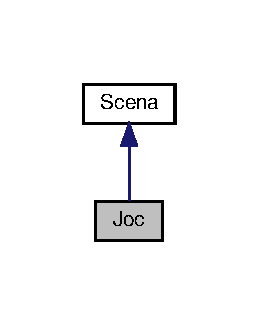
\includegraphics[width=124pt]{classJoc__inherit__graph}
\end{center}
\end{figure}


Diagrama de relaţii pentru Joc\+:
\nopagebreak
\begin{figure}[H]
\begin{center}
\leavevmode
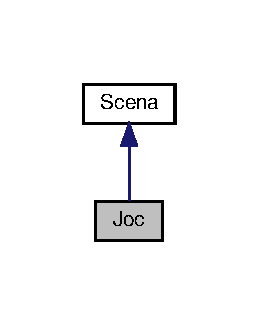
\includegraphics[width=124pt]{classJoc__coll__graph}
\end{center}
\end{figure}
\subsection*{Metode Publice}
\begin{DoxyCompactItemize}
\item 
\mbox{\Hypertarget{classJoc_ad0030f6756f45c5ac98a61d8094bf60e}\label{classJoc_ad0030f6756f45c5ac98a61d8094bf60e}} 
virtual void \hyperlink{classJoc_ad0030f6756f45c5ac98a61d8094bf60e}{iesire} (\hyperlink{classStadiulJocului}{Stadiul\+Jocului} \&) override
\begin{DoxyCompactList}\small\item\em Paraseste scena. \end{DoxyCompactList}\item 
virtual void \hyperlink{classJoc_a54976207efdeeb45b42fd639215b65e3}{incarca} (\hyperlink{classStadiulJocului}{Stadiul\+Jocului} \&) override
\item 
virtual bool \hyperlink{classJoc_ac78ae0ddb45250af612eb68de253861e}{incarcat\+\_\+deja} () override
\item 
virtual bool \hyperlink{classJoc_a5b8d52f928137512921eee184ca04fec}{itereaza} (\hyperlink{classStadiulJocului}{Stadiul\+Jocului} \&) override
\begin{DoxyCompactList}\small\item\em Executa functia la fiecare \textquotesingle{}desenare\textquotesingle{}. \end{DoxyCompactList}\end{DoxyCompactItemize}
\subsection*{Metode Private}
\begin{DoxyCompactItemize}
\item 
bool \hyperlink{classJoc_afd69d2cd19f6d2ac2b1a42a4685349e6}{muta\+\_\+omida} (\hyperlink{classStadiulJocului}{Stadiul\+Jocului} \&)
\item 
bool \hyperlink{classJoc_a0f90008558e8cbed6537b542f79ae55b}{pauza} (\hyperlink{classStadiulJocului}{Stadiul\+Jocului} \&)
\item 
\mbox{\Hypertarget{classJoc_a8e709a64cfcd3277975fb58f1bff3cd1}\label{classJoc_a8e709a64cfcd3277975fb58f1bff3cd1}} 
void \hyperlink{classJoc_a8e709a64cfcd3277975fb58f1bff3cd1}{pune\+\_\+scor} (\hyperlink{classStadiulJocului}{Stadiul\+Jocului} \&)
\begin{DoxyCompactList}\small\item\em Printeaza scorul curent pe capul omidei. \end{DoxyCompactList}\item 
\mbox{\Hypertarget{classJoc_a548406580ddf763a17061190fba3756e}\label{classJoc_a548406580ddf763a17061190fba3756e}} 
void \hyperlink{classJoc_a548406580ddf763a17061190fba3756e}{reseteaza\+\_\+teren} (\hyperlink{classStadiulJocului}{Stadiul\+Jocului} \&)
\begin{DoxyCompactList}\small\item\em Marcheaza totul Posibilitate\+Teren\+::\+G\+OL. \end{DoxyCompactList}\item 
bool \hyperlink{classJoc_afe57540f76b33492c721c14726a89d86}{verifica\+\_\+taste\+\_\+apasate} (\hyperlink{classStadiulJocului}{Stadiul\+Jocului} \&)
\begin{DoxyCompactList}\small\item\em Schimba Stadiul\+Jocului\+::noua\+\_\+directie\+\_\+a\+\_\+omizii in functie de tastele apasate. \end{DoxyCompactList}\end{DoxyCompactItemize}
\subsection*{Atribute Private}
\begin{DoxyCompactItemize}
\item 
long long \hyperlink{classJoc_a24e667d511404dd6479a86575f0969c2}{m\+\_\+timp\+\_\+asteptat} = 0\+LL
\item 
\hyperlink{main_8cpp_aea66a0d525bf9bfb9b61e9cc1ba0b752}{Tip\+Directie} \hyperlink{classJoc_af8df04a66ec45e3373dc6961b8f4a7cc}{noua\+\_\+directie\+\_\+a\+\_\+omizii} = Tip\+Directie\+::\+S\+US
\item 
\mbox{\Hypertarget{classJoc_a2b74a53ec4b88eb35c25da37c4cd4bb5}\label{classJoc_a2b74a53ec4b88eb35c25da37c4cd4bb5}} 
bool {\bfseries m\+\_\+incarcat\+\_\+deja} = false
\item 
\mbox{\Hypertarget{classJoc_afda2880b237b18b8bdd4f25c5817adb4}\label{classJoc_afda2880b237b18b8bdd4f25c5817adb4}} 
T\+T\+F\+\_\+\+Font $\ast$ \hyperlink{classJoc_afda2880b237b18b8bdd4f25c5817adb4}{m\+\_\+font} = nullptr
\begin{DoxyCompactList}\small\item\em Fontul folosit pentru a desena text pe ecran. \end{DoxyCompactList}\item 
\mbox{\Hypertarget{classJoc_ac92412a0e2de93936c4c600a7efe45f4}\label{classJoc_ac92412a0e2de93936c4c600a7efe45f4}} 
Mix\+\_\+\+Chunk $\ast$ \hyperlink{classJoc_ac92412a0e2de93936c4c600a7efe45f4}{m\+\_\+sunet\+\_\+frunza} = nullptr
\begin{DoxyCompactList}\small\item\em Sunetul redat de fiecare data cand omida mananca o frunza. \end{DoxyCompactList}\item 
\mbox{\Hypertarget{classJoc_aec45d2779304b9ee3ba5c3962a66323b}\label{classJoc_aec45d2779304b9ee3ba5c3962a66323b}} 
Mix\+\_\+\+Chunk $\ast$ \hyperlink{classJoc_aec45d2779304b9ee3ba5c3962a66323b}{m\+\_\+sunet\+\_\+powerup} = nullptr
\begin{DoxyCompactList}\small\item\em Sunetul redat de fiecare data cand omida mananca un powerup. \end{DoxyCompactList}\item 
\mbox{\Hypertarget{classJoc_a5b93484b69d553174400635eb36e3042}\label{classJoc_a5b93484b69d553174400635eb36e3042}} 
long long {\bfseries m\+\_\+timp\+\_\+powerup} = 0\+LL
\end{DoxyCompactItemize}


\subsection{Descriere Detaliată}
\hyperlink{classScena}{Scena} jocului in sine. 

Definiţia în linia 558 a fişierului main.\+cpp.



\subsection{Documentaţia Funcţiilor Membre}
\mbox{\Hypertarget{classJoc_a54976207efdeeb45b42fd639215b65e3}\label{classJoc_a54976207efdeeb45b42fd639215b65e3}} 
\index{Joc@{Joc}!incarca@{incarca}}
\index{incarca@{incarca}!Joc@{Joc}}
\subsubsection{\texorpdfstring{incarca()}{incarca()}}
{\footnotesize\ttfamily void Joc\+::incarca (\begin{DoxyParamCaption}\item[{\hyperlink{classStadiulJocului}{Stadiul\+Jocului} \&}]{ }\end{DoxyParamCaption})\hspace{0.3cm}{\ttfamily [override]}, {\ttfamily [virtual]}}

Initializeza scena. 

Implementează \hyperlink{classScena_a6f53a1dcef68084361dc8f9d56bbb8c0}{Scena}.



Definiţia în linia 1128 a fişierului main.\+cpp.



Referinţe global\+::desenator şi Stadiul\+Jocului\+::directia\+\_\+omizii.

\mbox{\Hypertarget{classJoc_ac78ae0ddb45250af612eb68de253861e}\label{classJoc_ac78ae0ddb45250af612eb68de253861e}} 
\index{Joc@{Joc}!incarcat\+\_\+deja@{incarcat\+\_\+deja}}
\index{incarcat\+\_\+deja@{incarcat\+\_\+deja}!Joc@{Joc}}
\subsubsection{\texorpdfstring{incarcat\+\_\+deja()}{incarcat\_deja()}}
{\footnotesize\ttfamily bool Joc\+::incarcat\+\_\+deja (\begin{DoxyParamCaption}{ }\end{DoxyParamCaption})\hspace{0.3cm}{\ttfamily [override]}, {\ttfamily [virtual]}}

Verifica daca scena curenta a fost incarcata deja. 

Implementează \hyperlink{classScena_ac8de771024795dffa0e5feb8dba881ff}{Scena}.



Definiţia în linia 1197 a fişierului main.\+cpp.

\mbox{\Hypertarget{classJoc_a5b8d52f928137512921eee184ca04fec}\label{classJoc_a5b8d52f928137512921eee184ca04fec}} 
\index{Joc@{Joc}!itereaza@{itereaza}}
\index{itereaza@{itereaza}!Joc@{Joc}}
\subsubsection{\texorpdfstring{itereaza()}{itereaza()}}
{\footnotesize\ttfamily bool Joc\+::itereaza (\begin{DoxyParamCaption}\item[{\hyperlink{classStadiulJocului}{Stadiul\+Jocului} \&}]{ }\end{DoxyParamCaption})\hspace{0.3cm}{\ttfamily [override]}, {\ttfamily [virtual]}}



Executa functia la fiecare \textquotesingle{}desenare\textquotesingle{}. 

\begin{DoxyReturn}{Întoarce}
Adevarat daca iterarea va continua, fals altfel. 
\end{DoxyReturn}


Implementează \hyperlink{classScena_a9e5fcc831ed410b5b2422231ede746ee}{Scena}.



Definiţia în linia 1200 a fişierului main.\+cpp.



Referinţe Stadiul\+Jocului\+::directia\+\_\+omizii, Stadiul\+Jocului\+::exista\+\_\+powerup, genereaza\+\_\+pozitie\+\_\+noua(), Punct\+::i, Punct\+::j, Stadiul\+Jocului\+::pozitie\+\_\+powerup, Stadiul\+Jocului\+::teren, Stadiul\+Jocului\+::timp\+\_\+asteptare\+\_\+maxim şi Stadiul\+Jocului\+::timp\+\_\+trecut.

\mbox{\Hypertarget{classJoc_afd69d2cd19f6d2ac2b1a42a4685349e6}\label{classJoc_afd69d2cd19f6d2ac2b1a42a4685349e6}} 
\index{Joc@{Joc}!muta\+\_\+omida@{muta\+\_\+omida}}
\index{muta\+\_\+omida@{muta\+\_\+omida}!Joc@{Joc}}
\subsubsection{\texorpdfstring{muta\+\_\+omida()}{muta\_omida()}}
{\footnotesize\ttfamily bool Joc\+::muta\+\_\+omida (\begin{DoxyParamCaption}\item[{\hyperlink{classStadiulJocului}{Stadiul\+Jocului} \&}]{stadiu }\end{DoxyParamCaption})\hspace{0.3cm}{\ttfamily [private]}}

Muta omida in directia setata de jucator.

\begin{DoxyReturn}{Întoarce}
Adevarat daca omida nu a murit, fals altfel. 
\end{DoxyReturn}


Definiţia în linia 992 a fişierului main.\+cpp.



Referinţe Stadiul\+Jocului\+::directia\+\_\+omizii, Punct\+::i, Stadiul\+Jocului\+::inaltime\+\_\+teren, Punct\+::j, Stadiul\+Jocului\+::lungime\+\_\+teren, Stadiul\+Jocului\+::pozitii\+\_\+omida şi Stadiul\+Jocului\+::teren.

\mbox{\Hypertarget{classJoc_a0f90008558e8cbed6537b542f79ae55b}\label{classJoc_a0f90008558e8cbed6537b542f79ae55b}} 
\index{Joc@{Joc}!pauza@{pauza}}
\index{pauza@{pauza}!Joc@{Joc}}
\subsubsection{\texorpdfstring{pauza()}{pauza()}}
{\footnotesize\ttfamily bool Joc\+::pauza (\begin{DoxyParamCaption}\item[{\hyperlink{classStadiulJocului}{Stadiul\+Jocului} \&}]{ }\end{DoxyParamCaption})\hspace{0.3cm}{\ttfamily [private]}}

Ruleaza cat timp jocul e in pauza.

\begin{DoxyReturn}{Întoarce}
Fals daca jucatorul a iesit din joc in timpul pauzei sau adevarat altfel. 
\end{DoxyReturn}


Definiţia în linia 1047 a fişierului main.\+cpp.



Referinţe a\+\_\+apasat(), global\+::taste\+\_\+apasate şi verifica\+\_\+evenimente().

\mbox{\Hypertarget{classJoc_afe57540f76b33492c721c14726a89d86}\label{classJoc_afe57540f76b33492c721c14726a89d86}} 
\index{Joc@{Joc}!verifica\+\_\+taste\+\_\+apasate@{verifica\+\_\+taste\+\_\+apasate}}
\index{verifica\+\_\+taste\+\_\+apasate@{verifica\+\_\+taste\+\_\+apasate}!Joc@{Joc}}
\subsubsection{\texorpdfstring{verifica\+\_\+taste\+\_\+apasate()}{verifica\_taste\_apasate()}}
{\footnotesize\ttfamily bool Joc\+::verifica\+\_\+taste\+\_\+apasate (\begin{DoxyParamCaption}\item[{\hyperlink{classStadiulJocului}{Stadiul\+Jocului} \&}]{stadiu }\end{DoxyParamCaption})\hspace{0.3cm}{\ttfamily [private]}}



Schimba Stadiul\+Jocului\+::noua\+\_\+directie\+\_\+a\+\_\+omizii in functie de tastele apasate. 

\begin{DoxyReturn}{Întoarce}
Fals daca jocul nu mai trebuie sa continue. 
\end{DoxyReturn}


Definiţia în linia 1097 a fişierului main.\+cpp.



Referinţe a\+\_\+apasat() şi Stadiul\+Jocului\+::directia\+\_\+omizii.



\subsection{Documentaţia Datelor Membre}
\mbox{\Hypertarget{classJoc_a24e667d511404dd6479a86575f0969c2}\label{classJoc_a24e667d511404dd6479a86575f0969c2}} 
\index{Joc@{Joc}!m\+\_\+timp\+\_\+asteptat@{m\+\_\+timp\+\_\+asteptat}}
\index{m\+\_\+timp\+\_\+asteptat@{m\+\_\+timp\+\_\+asteptat}!Joc@{Joc}}
\subsubsection{\texorpdfstring{m\+\_\+timp\+\_\+asteptat}{m\_timp\_asteptat}}
{\footnotesize\ttfamily long long Joc\+::m\+\_\+timp\+\_\+asteptat = 0\+LL\hspace{0.3cm}{\ttfamily [private]}}

Cand depaseste \hyperlink{classStadiulJocului_a4cdf9582b472e74980e1eee73ca94769}{Stadiul\+Jocului\+::timp\+\_\+asteptare\+\_\+maxim} omida trebuie mutata. 

Definiţia în linia 563 a fişierului main.\+cpp.

\mbox{\Hypertarget{classJoc_af8df04a66ec45e3373dc6961b8f4a7cc}\label{classJoc_af8df04a66ec45e3373dc6961b8f4a7cc}} 
\index{Joc@{Joc}!noua\+\_\+directie\+\_\+a\+\_\+omizii@{noua\+\_\+directie\+\_\+a\+\_\+omizii}}
\index{noua\+\_\+directie\+\_\+a\+\_\+omizii@{noua\+\_\+directie\+\_\+a\+\_\+omizii}!Joc@{Joc}}
\subsubsection{\texorpdfstring{noua\+\_\+directie\+\_\+a\+\_\+omizii}{noua\_directie\_a\_omizii}}
{\footnotesize\ttfamily \hyperlink{main_8cpp_aea66a0d525bf9bfb9b61e9cc1ba0b752}{Tip\+Directie} Joc\+::noua\+\_\+directie\+\_\+a\+\_\+omizii = Tip\+Directie\+::\+S\+US\hspace{0.3cm}{\ttfamily [private]}}

Pana cand omida trebuie mutata actualizeaza directia. De exemplu, jucatorul apasa tasta UP, dar dupa apasa D\+O\+WN fara ca \hyperlink{classJoc_a24e667d511404dd6479a86575f0969c2}{Joc\+::m\+\_\+timp\+\_\+asteptat} sa fi depasit \hyperlink{classStadiulJocului_a4cdf9582b472e74980e1eee73ca94769}{Stadiul\+Jocului\+::timp\+\_\+asteptare\+\_\+maxim}. Cand omida trebuie mutata actualizeaza \hyperlink{classStadiulJocului_a79d2c301f57a7fc525534994ffd7057e}{Stadiul\+Jocului\+::directia\+\_\+omizii} cu directia noua. 

Definiţia în linia 571 a fişierului main.\+cpp.



Documentaţia pentru această clasă a fost generată din fişierul\+:\begin{DoxyCompactItemize}
\item 
\hyperlink{main_8cpp}{main.\+cpp}\end{DoxyCompactItemize}

\hypertarget{classMeniuFinal}{}\section{Referinţă la clasa Meniu\+Final}
\label{classMeniuFinal}\index{Meniu\+Final@{Meniu\+Final}}


Meniul care va fi afisat dupa terminarea unui joc.  




Diagrama de relaţii pentru Meniu\+Final
\nopagebreak
\begin{figure}[H]
\begin{center}
\leavevmode
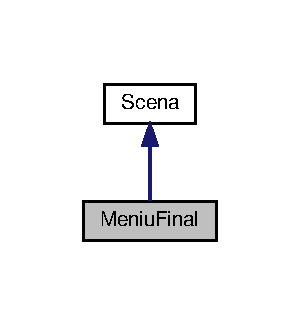
\includegraphics[width=144pt]{classMeniuFinal__inherit__graph}
\end{center}
\end{figure}


Diagrama de relaţii pentru Meniu\+Final\+:
\nopagebreak
\begin{figure}[H]
\begin{center}
\leavevmode
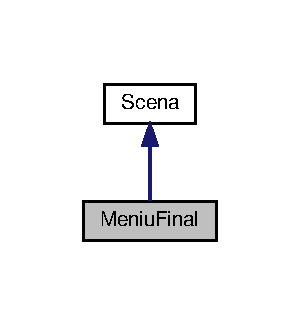
\includegraphics[width=144pt]{classMeniuFinal__coll__graph}
\end{center}
\end{figure}
\subsection*{Metode Publice}
\begin{DoxyCompactItemize}
\item 
\mbox{\Hypertarget{classMeniuFinal_a1effd96032aadf141533119115dbbe91}\label{classMeniuFinal_a1effd96032aadf141533119115dbbe91}} 
virtual void \hyperlink{classMeniuFinal_a1effd96032aadf141533119115dbbe91}{iesire} (\hyperlink{classStadiulJocului}{Stadiul\+Jocului} \&) override
\begin{DoxyCompactList}\small\item\em Paraseste scena. \end{DoxyCompactList}\item 
virtual void \hyperlink{classMeniuFinal_a4a1f2a872c6d0cef0e3f0a8e1545f5de}{incarca} (\hyperlink{classStadiulJocului}{Stadiul\+Jocului} \&) override
\item 
virtual bool \hyperlink{classMeniuFinal_a72edd47d4783b321124d7d7af74b9ef8}{incarcat\+\_\+deja} () override
\item 
virtual bool \hyperlink{classMeniuFinal_a9ee1a22d9df62f0828961d38e05f8aa4}{itereaza} (\hyperlink{classStadiulJocului}{Stadiul\+Jocului} \&) override
\begin{DoxyCompactList}\small\item\em Executa functia la fiecare \textquotesingle{}desenare\textquotesingle{}. \end{DoxyCompactList}\end{DoxyCompactItemize}
\subsection*{Metode Private}
\begin{DoxyCompactItemize}
\item 
\mbox{\Hypertarget{classMeniuFinal_a663058fca13b16c502d22ac4ee488cf0}\label{classMeniuFinal_a663058fca13b16c502d22ac4ee488cf0}} 
void {\bfseries citeste\+\_\+istoric} ()
\end{DoxyCompactItemize}
\subsection*{Atribute Private}
\begin{DoxyCompactItemize}
\item 
\mbox{\Hypertarget{classMeniuFinal_aedde998b4a8c6b468d7dc1a4c5af4cbc}\label{classMeniuFinal_aedde998b4a8c6b468d7dc1a4c5af4cbc}} 
bool {\bfseries m\+\_\+incarcat\+\_\+deja} = false
\item 
\mbox{\Hypertarget{classMeniuFinal_a8ca418faf68fa155bc809a325479a02a}\label{classMeniuFinal_a8ca418faf68fa155bc809a325479a02a}} 
T\+T\+F\+\_\+\+Font $\ast$ {\bfseries m\+\_\+font} = nullptr
\item 
\mbox{\Hypertarget{classMeniuFinal_a79c050764da86c93f5554265a7567036}\label{classMeniuFinal_a79c050764da86c93f5554265a7567036}} 
S\+D\+L\+\_\+\+Texture $\ast$ {\bfseries m\+\_\+text} = nullptr
\item 
\mbox{\Hypertarget{classMeniuFinal_a3d0af1b8d2ce9ba4e2013ddb68f5786f}\label{classMeniuFinal_a3d0af1b8d2ce9ba4e2013ddb68f5786f}} 
S\+D\+L\+\_\+\+Texture $\ast$ {\bfseries m\+\_\+text\+\_\+scor\+\_\+maxim} = nullptr
\item 
std\+::ifstream \hyperlink{classMeniuFinal_a995e013192e1bed67332f0d54ae2b482}{m\+\_\+istoric} \{\}
\begin{DoxyCompactList}\small\item\em Fisierul in care sunt stocate toate scorurile. \end{DoxyCompactList}\item 
\mbox{\Hypertarget{classMeniuFinal_a9dd63e1fb07a20c48cec529f794945a8}\label{classMeniuFinal_a9dd63e1fb07a20c48cec529f794945a8}} 
int {\bfseries m\+\_\+scor\+\_\+maxim} \{ 0 \}
\item 
\mbox{\Hypertarget{classMeniuFinal_a45688213631c7266bb329f301523dfb0}\label{classMeniuFinal_a45688213631c7266bb329f301523dfb0}} 
std\+::string {\bfseries m\+\_\+numele\+\_\+scorului\+\_\+maxim} \{ \char`\"{}\char`\"{} \}
\item 
\mbox{\Hypertarget{classMeniuFinal_aa940eaec12a96d8a9037cd698c5c2baa}\label{classMeniuFinal_aa940eaec12a96d8a9037cd698c5c2baa}} 
std\+::string {\bfseries m\+\_\+anul\+\_\+scorului\+\_\+maxim} \{ \char`\"{}\char`\"{} \}
\item 
\mbox{\Hypertarget{classMeniuFinal_a17611b8f7fb8442187fced397c26875a}\label{classMeniuFinal_a17611b8f7fb8442187fced397c26875a}} 
std\+::string {\bfseries m\+\_\+luna\+\_\+scorului\+\_\+maxim} \{ \char`\"{}\char`\"{} \}
\item 
\mbox{\Hypertarget{classMeniuFinal_a3fd4cb6ddc4cfd8bb84cfad734137d8c}\label{classMeniuFinal_a3fd4cb6ddc4cfd8bb84cfad734137d8c}} 
std\+::string {\bfseries m\+\_\+ziua\+\_\+scorului\+\_\+maxim} \{ \char`\"{}\char`\"{} \}
\item 
\mbox{\Hypertarget{classMeniuFinal_a7e6102d7ba03592db9af4d2ff8a3c0de}\label{classMeniuFinal_a7e6102d7ba03592db9af4d2ff8a3c0de}} 
bool {\bfseries m\+\_\+are\+\_\+scor\+\_\+maxim} \{ false \}
\item 
\mbox{\Hypertarget{classMeniuFinal_af0bf7286afbfcf28139aed5fd426a1c8}\label{classMeniuFinal_af0bf7286afbfcf28139aed5fd426a1c8}} 
std\+::string {\bfseries m\+\_\+nume\+\_\+curent} \{ \char`\"{}N\+U\+ME\char`\"{} \}
\item 
\mbox{\Hypertarget{classMeniuFinal_a9c703f1f5632ca0acfef05a7030647b5}\label{classMeniuFinal_a9c703f1f5632ca0acfef05a7030647b5}} 
S\+D\+L\+\_\+\+Texture $\ast$ {\bfseries m\+\_\+text\+\_\+nume\+\_\+curent} \{ nullptr \}
\end{DoxyCompactItemize}


\subsection{Descriere Detaliată}
Meniul care va fi afisat dupa terminarea unui joc. 

Definiţia în linia 668 a fişierului main.\+cpp.



\subsection{Documentaţia Funcţiilor Membre}
\mbox{\Hypertarget{classMeniuFinal_a4a1f2a872c6d0cef0e3f0a8e1545f5de}\label{classMeniuFinal_a4a1f2a872c6d0cef0e3f0a8e1545f5de}} 
\index{Meniu\+Final@{Meniu\+Final}!incarca@{incarca}}
\index{incarca@{incarca}!Meniu\+Final@{Meniu\+Final}}
\subsubsection{\texorpdfstring{incarca()}{incarca()}}
{\footnotesize\ttfamily void Meniu\+Final\+::incarca (\begin{DoxyParamCaption}\item[{\hyperlink{classStadiulJocului}{Stadiul\+Jocului} \&}]{ }\end{DoxyParamCaption})\hspace{0.3cm}{\ttfamily [override]}, {\ttfamily [virtual]}}

Initializeza scena. 

Implementează \hyperlink{classScena_a6f53a1dcef68084361dc8f9d56bbb8c0}{Scena}.



Definiţia în linia 1436 a fişierului main.\+cpp.



Referinţe global\+::desenator şi Stadiul\+Jocului\+::scor.

\mbox{\Hypertarget{classMeniuFinal_a72edd47d4783b321124d7d7af74b9ef8}\label{classMeniuFinal_a72edd47d4783b321124d7d7af74b9ef8}} 
\index{Meniu\+Final@{Meniu\+Final}!incarcat\+\_\+deja@{incarcat\+\_\+deja}}
\index{incarcat\+\_\+deja@{incarcat\+\_\+deja}!Meniu\+Final@{Meniu\+Final}}
\subsubsection{\texorpdfstring{incarcat\+\_\+deja()}{incarcat\_deja()}}
{\footnotesize\ttfamily bool Meniu\+Final\+::incarcat\+\_\+deja (\begin{DoxyParamCaption}{ }\end{DoxyParamCaption})\hspace{0.3cm}{\ttfamily [override]}, {\ttfamily [virtual]}}

Verifica daca scena curenta a fost incarcata deja. 

Implementează \hyperlink{classScena_ac8de771024795dffa0e5feb8dba881ff}{Scena}.



Definiţia în linia 1498 a fişierului main.\+cpp.

\mbox{\Hypertarget{classMeniuFinal_a9ee1a22d9df62f0828961d38e05f8aa4}\label{classMeniuFinal_a9ee1a22d9df62f0828961d38e05f8aa4}} 
\index{Meniu\+Final@{Meniu\+Final}!itereaza@{itereaza}}
\index{itereaza@{itereaza}!Meniu\+Final@{Meniu\+Final}}
\subsubsection{\texorpdfstring{itereaza()}{itereaza()}}
{\footnotesize\ttfamily bool Meniu\+Final\+::itereaza (\begin{DoxyParamCaption}\item[{\hyperlink{classStadiulJocului}{Stadiul\+Jocului} \&}]{ }\end{DoxyParamCaption})\hspace{0.3cm}{\ttfamily [override]}, {\ttfamily [virtual]}}



Executa functia la fiecare \textquotesingle{}desenare\textquotesingle{}. 

\begin{DoxyReturn}{Întoarce}
Adevarat daca iterarea va continua, fals altfel. 
\end{DoxyReturn}


Implementează \hyperlink{classScena_a9e5fcc831ed410b5b2422231ede746ee}{Scena}.



Definiţia în linia 1528 a fişierului main.\+cpp.



Referinţe a\+\_\+apasat(), global\+::scene şi global\+::taste\+\_\+apasate.



\subsection{Documentaţia Datelor Membre}
\mbox{\Hypertarget{classMeniuFinal_a995e013192e1bed67332f0d54ae2b482}\label{classMeniuFinal_a995e013192e1bed67332f0d54ae2b482}} 
\index{Meniu\+Final@{Meniu\+Final}!m\+\_\+istoric@{m\+\_\+istoric}}
\index{m\+\_\+istoric@{m\+\_\+istoric}!Meniu\+Final@{Meniu\+Final}}
\subsubsection{\texorpdfstring{m\+\_\+istoric}{m\_istoric}}
{\footnotesize\ttfamily std\+::ifstream Meniu\+Final\+::m\+\_\+istoric \{\}\hspace{0.3cm}{\ttfamily [private]}}



Fisierul in care sunt stocate toate scorurile. 

Istoricul are forma\+: Nume Jucator Luna zi An Scor 

Definiţia în linia 684 a fişierului main.\+cpp.



Documentaţia pentru această clasă a fost generată din fişierul\+:\begin{DoxyCompactItemize}
\item 
\hyperlink{main_8cpp}{main.\+cpp}\end{DoxyCompactItemize}

\hypertarget{classMeniuStart}{}\section{Referinţă la clasa Meniu\+Start}
\label{classMeniuStart}\index{Meniu\+Start@{Meniu\+Start}}


Defineste meniul afisat la deschiderea jocului.  




Diagrama de relaţii pentru Meniu\+Start
\nopagebreak
\begin{figure}[H]
\begin{center}
\leavevmode
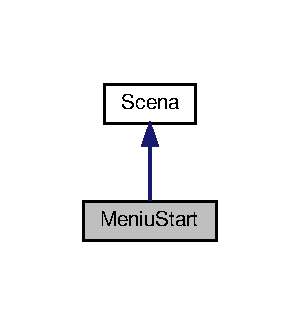
\includegraphics[width=144pt]{classMeniuStart__inherit__graph}
\end{center}
\end{figure}


Diagrama de relaţii pentru Meniu\+Start\+:
\nopagebreak
\begin{figure}[H]
\begin{center}
\leavevmode
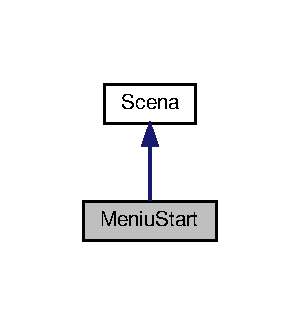
\includegraphics[width=144pt]{classMeniuStart__coll__graph}
\end{center}
\end{figure}
\subsection*{Metode Publice}
\begin{DoxyCompactItemize}
\item 
\mbox{\Hypertarget{classMeniuStart_abfc0ef10adadd6f9756996fc7c61bf76}\label{classMeniuStart_abfc0ef10adadd6f9756996fc7c61bf76}} 
virtual void \hyperlink{classMeniuStart_abfc0ef10adadd6f9756996fc7c61bf76}{iesire} (\hyperlink{classStadiulJocului}{Stadiul\+Jocului} \&) override
\begin{DoxyCompactList}\small\item\em Paraseste scena. \end{DoxyCompactList}\item 
virtual void \hyperlink{classMeniuStart_afb59dcb21968a6ccd685a6c9c0d6a0c1}{incarca} (\hyperlink{classStadiulJocului}{Stadiul\+Jocului} \&) override
\item 
virtual bool \hyperlink{classMeniuStart_a76d8d1b449800060994971ea9df75fd3}{incarcat\+\_\+deja} () override
\item 
virtual bool \hyperlink{classMeniuStart_a35a84c537eca90b76697d1bef88216e5}{itereaza} (\hyperlink{classStadiulJocului}{Stadiul\+Jocului} \&) override
\begin{DoxyCompactList}\small\item\em Executa functia la fiecare \textquotesingle{}desenare\textquotesingle{}. \end{DoxyCompactList}\end{DoxyCompactItemize}
\subsection*{Tipuri Private}
\begin{DoxyCompactItemize}
\item 
\mbox{\Hypertarget{classMeniuStart_a9c31d6c8b52efb87116aac4b176f8375}\label{classMeniuStart_a9c31d6c8b52efb87116aac4b176f8375}} 
enum {\bfseries tip\+\_\+meniu} \{ {\bfseries S\+T\+A\+R\+T\+\_\+\+J\+OC} = 0, 
{\bfseries I\+E\+S\+I\+RE}, 
{\bfseries N\+R\+\_\+\+M\+E\+N\+I\+U\+RI}
 \}
\end{DoxyCompactItemize}
\subsection*{Metode Private}
\begin{DoxyCompactItemize}
\item 
\mbox{\Hypertarget{classMeniuStart_ae81aee43c415d5ea2f07469baa2fcfc1}\label{classMeniuStart_ae81aee43c415d5ea2f07469baa2fcfc1}} 
bool {\bfseries click\+\_\+in\+\_\+meniu} ()
\item 
\mbox{\Hypertarget{classMeniuStart_a046f60fb2d3a67db5cef26376c69150e}\label{classMeniuStart_a046f60fb2d3a67db5cef26376c69150e}} 
bool {\bfseries verifica\+\_\+evenimente} (\hyperlink{classStadiulJocului}{Stadiul\+Jocului} \&)
\end{DoxyCompactItemize}
\subsection*{Atribute Private}
\begin{DoxyCompactItemize}
\item 
\mbox{\Hypertarget{classMeniuStart_a9d934fb5c51907f5f0bce6d259cdeb24}\label{classMeniuStart_a9d934fb5c51907f5f0bce6d259cdeb24}} 
bool {\bfseries m\+\_\+incarcat} = false
\item 
\mbox{\Hypertarget{classMeniuStart_aea1b80044a1dce077fd9bd052bbfe279}\label{classMeniuStart_aea1b80044a1dce077fd9bd052bbfe279}} 
tip\+\_\+meniu {\bfseries m\+\_\+meniu\+\_\+selectat} = tip\+\_\+meniu\+::\+S\+T\+A\+R\+T\+\_\+\+J\+OC
\item 
\mbox{\Hypertarget{classMeniuStart_a0428348c2459b05e54c32ee3835a80cf}\label{classMeniuStart_a0428348c2459b05e54c32ee3835a80cf}} 
S\+D\+L\+\_\+\+Rect {\bfseries m\+\_\+dreptunghi\+\_\+meniu} \mbox{[}N\+R\+\_\+\+M\+E\+N\+I\+U\+RI\mbox{]}
\item 
\mbox{\Hypertarget{classMeniuStart_acd083e350cda462b27e3cfccc2ca4298}\label{classMeniuStart_acd083e350cda462b27e3cfccc2ca4298}} 
S\+D\+L\+\_\+\+Texture $\ast$ {\bfseries m\+\_\+textura\+\_\+meniu} \mbox{[}N\+R\+\_\+\+M\+E\+N\+I\+U\+RI\mbox{]}
\item 
\mbox{\Hypertarget{classMeniuStart_a6982327ecd2eb251a25da2651b1ee80a}\label{classMeniuStart_a6982327ecd2eb251a25da2651b1ee80a}} 
T\+T\+F\+\_\+\+Font $\ast$ {\bfseries m\+\_\+font} = nullptr
\item 
\mbox{\Hypertarget{classMeniuStart_a93aae50a78dc2df745728a2e8b6bbb11}\label{classMeniuStart_a93aae50a78dc2df745728a2e8b6bbb11}} 
const char $\ast$ {\bfseries m\+\_\+meniu\+\_\+text} \mbox{[}N\+R\+\_\+\+M\+E\+N\+I\+U\+RI\mbox{]}
\item 
\mbox{\Hypertarget{classMeniuStart_a9b6b148717c5fd9f860bc046ecac255c}\label{classMeniuStart_a9b6b148717c5fd9f860bc046ecac255c}} 
const S\+D\+L\+\_\+\+Color {\bfseries m\+\_\+culoare\+\_\+background\+\_\+meniu} = \{ 153, 51, 153, 255 \}
\end{DoxyCompactItemize}


\subsection{Descriere Detaliată}
Defineste meniul afisat la deschiderea jocului. 

Definiţia în linia 631 a fişierului main.\+cpp.



\subsection{Documentaţia Funcţiilor Membre}
\mbox{\Hypertarget{classMeniuStart_afb59dcb21968a6ccd685a6c9c0d6a0c1}\label{classMeniuStart_afb59dcb21968a6ccd685a6c9c0d6a0c1}} 
\index{Meniu\+Start@{Meniu\+Start}!incarca@{incarca}}
\index{incarca@{incarca}!Meniu\+Start@{Meniu\+Start}}
\subsubsection{\texorpdfstring{incarca()}{incarca()}}
{\footnotesize\ttfamily void Meniu\+Start\+::incarca (\begin{DoxyParamCaption}\item[{\hyperlink{classStadiulJocului}{Stadiul\+Jocului} \&}]{ }\end{DoxyParamCaption})\hspace{0.3cm}{\ttfamily [override]}, {\ttfamily [virtual]}}

Initializeza scena. 

Implementează \hyperlink{classScena_a6f53a1dcef68084361dc8f9d56bbb8c0}{Scena}.



Definiţia în linia 1304 a fişierului main.\+cpp.



Referinţe global\+::desenator, Punct\+::i, global\+::inaltime şi global\+::lungime.

\mbox{\Hypertarget{classMeniuStart_a76d8d1b449800060994971ea9df75fd3}\label{classMeniuStart_a76d8d1b449800060994971ea9df75fd3}} 
\index{Meniu\+Start@{Meniu\+Start}!incarcat\+\_\+deja@{incarcat\+\_\+deja}}
\index{incarcat\+\_\+deja@{incarcat\+\_\+deja}!Meniu\+Start@{Meniu\+Start}}
\subsubsection{\texorpdfstring{incarcat\+\_\+deja()}{incarcat\_deja()}}
{\footnotesize\ttfamily bool Meniu\+Start\+::incarcat\+\_\+deja (\begin{DoxyParamCaption}{ }\end{DoxyParamCaption})\hspace{0.3cm}{\ttfamily [override]}, {\ttfamily [virtual]}}

Verifica daca scena curenta a fost incarcata deja. 

Implementează \hyperlink{classScena_ac8de771024795dffa0e5feb8dba881ff}{Scena}.



Definiţia în linia 1335 a fişierului main.\+cpp.

\mbox{\Hypertarget{classMeniuStart_a35a84c537eca90b76697d1bef88216e5}\label{classMeniuStart_a35a84c537eca90b76697d1bef88216e5}} 
\index{Meniu\+Start@{Meniu\+Start}!itereaza@{itereaza}}
\index{itereaza@{itereaza}!Meniu\+Start@{Meniu\+Start}}
\subsubsection{\texorpdfstring{itereaza()}{itereaza()}}
{\footnotesize\ttfamily bool Meniu\+Start\+::itereaza (\begin{DoxyParamCaption}\item[{\hyperlink{classStadiulJocului}{Stadiul\+Jocului} \&}]{ }\end{DoxyParamCaption})\hspace{0.3cm}{\ttfamily [override]}, {\ttfamily [virtual]}}



Executa functia la fiecare \textquotesingle{}desenare\textquotesingle{}. 

\begin{DoxyReturn}{Întoarce}
Adevarat daca iterarea va continua, fals altfel. 
\end{DoxyReturn}


Implementează \hyperlink{classScena_a9e5fcc831ed410b5b2422231ede746ee}{Scena}.



Definiţia în linia 1338 a fişierului main.\+cpp.



Referinţe a\+\_\+apasat(), global\+::desenator, global\+::fereastra\+\_\+inchisa, Punct\+::i, Stadiul\+Jocului\+::inaltime\+\_\+textura, Stadiul\+Jocului\+::lungime\+\_\+textura şi verifica\+\_\+evenimente().



Documentaţia pentru această clasă a fost generată din fişierul\+:\begin{DoxyCompactItemize}
\item 
\hyperlink{main_8cpp}{main.\+cpp}\end{DoxyCompactItemize}

\hypertarget{structPunct}{}\section{Referinţă la structura Punct}
\label{structPunct}\index{Punct@{Punct}}
\subsection*{Metode Publice}
\begin{DoxyCompactItemize}
\item 
\hyperlink{structPunct_a04070b9c9925f7f4a117ecec3d3338af}{Punct} ()=default
\item 
\hyperlink{structPunct_a2ff34bc87cb16eae3d747ff63d51bff0}{Punct} (int t\+\_\+i, int t\+\_\+j)
\item 
\hyperlink{structPunct_afa529a8fdfbc33103f357f754ba4105e}{Punct} (const \hyperlink{structPunct}{Punct} \&)=default
\end{DoxyCompactItemize}
\subsection*{Atribute Publice}
\begin{DoxyCompactItemize}
\item 
\mbox{\Hypertarget{structPunct_a28bb6f2facdfadbf7e19d651c526a646}\label{structPunct_a28bb6f2facdfadbf7e19d651c526a646}} 
int \hyperlink{structPunct_a28bb6f2facdfadbf7e19d651c526a646}{i} \{ 0 \}
\begin{DoxyCompactList}\small\item\em Linia in matrice. \end{DoxyCompactList}\item 
\mbox{\Hypertarget{structPunct_a065a30931a1d15d6f6c638c4888d254e}\label{structPunct_a065a30931a1d15d6f6c638c4888d254e}} 
int \hyperlink{structPunct_a065a30931a1d15d6f6c638c4888d254e}{j} \{ 0 \}
\begin{DoxyCompactList}\small\item\em Coloana in matrice. \end{DoxyCompactList}\end{DoxyCompactItemize}


\subsection{Descriere Detaliată}
O structura ajutatoare pentru a reprezenta o pozitie in matricea jocului. 

Definiţia în linia 289 a fişierului main.\+cpp.



\subsection{Documentaţia pentru Constructori şi Destructori}
\mbox{\Hypertarget{structPunct_a04070b9c9925f7f4a117ecec3d3338af}\label{structPunct_a04070b9c9925f7f4a117ecec3d3338af}} 
\index{Punct@{Punct}!Punct@{Punct}}
\index{Punct@{Punct}!Punct@{Punct}}
\subsubsection{\texorpdfstring{Punct()}{Punct()}\hspace{0.1cm}{\footnotesize\ttfamily [1/3]}}
{\footnotesize\ttfamily Punct\+::\+Punct (\begin{DoxyParamCaption}{ }\end{DoxyParamCaption})\hspace{0.3cm}{\ttfamily [default]}}

Vrem ca o variabila de tipul \hyperlink{structPunct}{Punct} sa aiba valorile initiale i = 0 si j = 0 asa ca nu ar trebui modificat nimic in constructor.

Exemplu\+: 
\begin{DoxyCode}
\hyperlink{structPunct}{Punct} a;
a.\hyperlink{structPunct_a28bb6f2facdfadbf7e19d651c526a646}{i} == 0; \textcolor{comment}{// adevarat}
a.\hyperlink{structPunct_a065a30931a1d15d6f6c638c4888d254e}{j} == 0; \textcolor{comment}{// adevarat}
\end{DoxyCode}
 

Semnalat de Punct().

\mbox{\Hypertarget{structPunct_a2ff34bc87cb16eae3d747ff63d51bff0}\label{structPunct_a2ff34bc87cb16eae3d747ff63d51bff0}} 
\index{Punct@{Punct}!Punct@{Punct}}
\index{Punct@{Punct}!Punct@{Punct}}
\subsubsection{\texorpdfstring{Punct()}{Punct()}\hspace{0.1cm}{\footnotesize\ttfamily [2/3]}}
{\footnotesize\ttfamily Punct\+::\+Punct (\begin{DoxyParamCaption}\item[{int}]{t\+\_\+i,  }\item[{int}]{t\+\_\+j }\end{DoxyParamCaption})\hspace{0.3cm}{\ttfamily [inline]}}

Putem declara un punct si cu valori customizate pe loc, exemplu\+: 
\begin{DoxyCode}
\hyperlink{structPunct}{Punct} a\{ 2, 3 \}; \textcolor{comment}{// a.i va fi 2 si a.j va fi 3}
\hyperlink{structPunct}{Punct} b(2, 3); \textcolor{comment}{// la fel ca a}
\end{DoxyCode}
 

Definiţia în linia 319 a fişierului main.\+cpp.



Referinţe j şi Punct().

\mbox{\Hypertarget{structPunct_afa529a8fdfbc33103f357f754ba4105e}\label{structPunct_afa529a8fdfbc33103f357f754ba4105e}} 
\index{Punct@{Punct}!Punct@{Punct}}
\index{Punct@{Punct}!Punct@{Punct}}
\subsubsection{\texorpdfstring{Punct()}{Punct()}\hspace{0.1cm}{\footnotesize\ttfamily [3/3]}}
{\footnotesize\ttfamily Punct\+::\+Punct (\begin{DoxyParamCaption}\item[{const \hyperlink{structPunct}{Punct} \&}]{ }\end{DoxyParamCaption})\hspace{0.3cm}{\ttfamily [default]}}

Declarat pentru a putea copia valorile unui punct in alta variabila, exemplu\+: 
\begin{DoxyCode}
\hyperlink{structPunct}{Punct} a\{ 2, 3 \};
\hyperlink{structPunct}{Punct} b\{ 5, 6 \};
b = a; \textcolor{comment}{// acum b.i = 2 si b.j = 3}
\end{DoxyCode}
 

Documentaţia pentru această structură a fost generată din fişierul\+:\begin{DoxyCompactItemize}
\item 
\hyperlink{main_8cpp}{main.\+cpp}\end{DoxyCompactItemize}

\hypertarget{classScena}{}\section{Referinţă la clasa Scena}
\label{classScena}\index{Scena@{Scena}}


Interfata pentru toate scenele.  




Diagrama de relaţii pentru Scena
\nopagebreak
\begin{figure}[H]
\begin{center}
\leavevmode
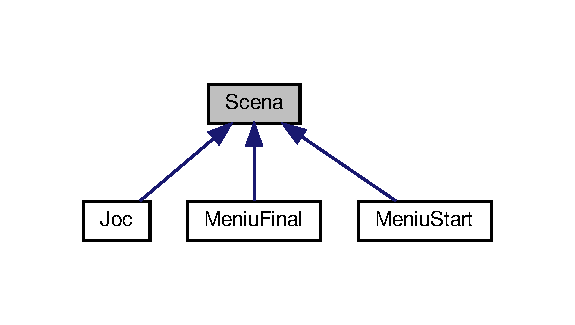
\includegraphics[width=276pt]{classScena__inherit__graph}
\end{center}
\end{figure}
\subsection*{Metode Publice}
\begin{DoxyCompactItemize}
\item 
virtual void \hyperlink{classScena_a6f53a1dcef68084361dc8f9d56bbb8c0}{incarca} (\hyperlink{classStadiulJocului}{Stadiul\+Jocului} \&)=0
\item 
virtual bool \hyperlink{classScena_ac8de771024795dffa0e5feb8dba881ff}{incarcat\+\_\+deja} ()=0
\item 
\mbox{\Hypertarget{classScena_a6c1ec6a3ed0acc18f71e9b8a2c077f7a}\label{classScena_a6c1ec6a3ed0acc18f71e9b8a2c077f7a}} 
virtual void \hyperlink{classScena_a6c1ec6a3ed0acc18f71e9b8a2c077f7a}{iesire} (\hyperlink{classStadiulJocului}{Stadiul\+Jocului} \&)=0
\begin{DoxyCompactList}\small\item\em Paraseste scena. \end{DoxyCompactList}\item 
virtual bool \hyperlink{classScena_a9e5fcc831ed410b5b2422231ede746ee}{itereaza} (\hyperlink{classStadiulJocului}{Stadiul\+Jocului} \&)=0
\begin{DoxyCompactList}\small\item\em Executa functia la fiecare \textquotesingle{}desenare\textquotesingle{}. \end{DoxyCompactList}\end{DoxyCompactItemize}


\subsection{Descriere Detaliată}
Interfata pentru toate scenele. 

Definiţia în linia 530 a fişierului main.\+cpp.



\subsection{Documentaţia Funcţiilor Membre}
\mbox{\Hypertarget{classScena_a6f53a1dcef68084361dc8f9d56bbb8c0}\label{classScena_a6f53a1dcef68084361dc8f9d56bbb8c0}} 
\index{Scena@{Scena}!incarca@{incarca}}
\index{incarca@{incarca}!Scena@{Scena}}
\subsubsection{\texorpdfstring{incarca()}{incarca()}}
{\footnotesize\ttfamily virtual void Scena\+::incarca (\begin{DoxyParamCaption}\item[{\hyperlink{classStadiulJocului}{Stadiul\+Jocului} \&}]{ }\end{DoxyParamCaption})\hspace{0.3cm}{\ttfamily [pure virtual]}}

Initializeza scena. 

Implementat în \hyperlink{classMeniuFinal_a4a1f2a872c6d0cef0e3f0a8e1545f5de}{Meniu\+Final}, \hyperlink{classMeniuStart_afb59dcb21968a6ccd685a6c9c0d6a0c1}{Meniu\+Start} şi \hyperlink{classJoc_a54976207efdeeb45b42fd639215b65e3}{Joc}.

\mbox{\Hypertarget{classScena_ac8de771024795dffa0e5feb8dba881ff}\label{classScena_ac8de771024795dffa0e5feb8dba881ff}} 
\index{Scena@{Scena}!incarcat\+\_\+deja@{incarcat\+\_\+deja}}
\index{incarcat\+\_\+deja@{incarcat\+\_\+deja}!Scena@{Scena}}
\subsubsection{\texorpdfstring{incarcat\+\_\+deja()}{incarcat\_deja()}}
{\footnotesize\ttfamily virtual bool Scena\+::incarcat\+\_\+deja (\begin{DoxyParamCaption}{ }\end{DoxyParamCaption})\hspace{0.3cm}{\ttfamily [pure virtual]}}

Verifica daca scena curenta a fost incarcata deja. 

Implementat în \hyperlink{classMeniuFinal_a72edd47d4783b321124d7d7af74b9ef8}{Meniu\+Final}, \hyperlink{classMeniuStart_a76d8d1b449800060994971ea9df75fd3}{Meniu\+Start} şi \hyperlink{classJoc_ac78ae0ddb45250af612eb68de253861e}{Joc}.

\mbox{\Hypertarget{classScena_a9e5fcc831ed410b5b2422231ede746ee}\label{classScena_a9e5fcc831ed410b5b2422231ede746ee}} 
\index{Scena@{Scena}!itereaza@{itereaza}}
\index{itereaza@{itereaza}!Scena@{Scena}}
\subsubsection{\texorpdfstring{itereaza()}{itereaza()}}
{\footnotesize\ttfamily virtual bool Scena\+::itereaza (\begin{DoxyParamCaption}\item[{\hyperlink{classStadiulJocului}{Stadiul\+Jocului} \&}]{ }\end{DoxyParamCaption})\hspace{0.3cm}{\ttfamily [pure virtual]}}



Executa functia la fiecare \textquotesingle{}desenare\textquotesingle{}. 

\begin{DoxyReturn}{Întoarce}
Adevarat daca iterarea va continua, fals altfel. 
\end{DoxyReturn}


Implementat în \hyperlink{classMeniuFinal_a9ee1a22d9df62f0828961d38e05f8aa4}{Meniu\+Final}, \hyperlink{classMeniuStart_a35a84c537eca90b76697d1bef88216e5}{Meniu\+Start} şi \hyperlink{classJoc_a5b8d52f928137512921eee184ca04fec}{Joc}.



Documentaţia pentru această clasă a fost generată din fişierul\+:\begin{DoxyCompactItemize}
\item 
\hyperlink{main_8cpp}{main.\+cpp}\end{DoxyCompactItemize}

\hypertarget{classStadiulJocului}{}\section{Referinţă la clasa Stadiul\+Jocului}
\label{classStadiulJocului}\index{Stadiul\+Jocului@{Stadiul\+Jocului}}


Contine toata informatia de care avem nevoie in timpul jocului.  




Diagrama de relaţii pentru Stadiul\+Jocului\+:
\nopagebreak
\begin{figure}[H]
\begin{center}
\leavevmode
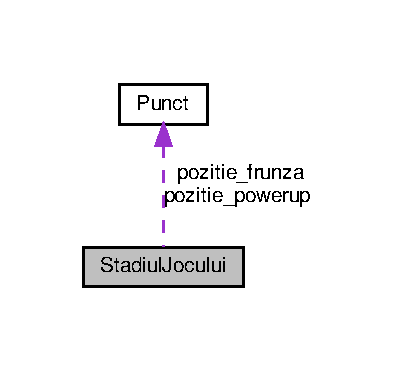
\includegraphics[width=190pt]{classStadiulJocului__coll__graph}
\end{center}
\end{figure}
\subsection*{Atribute Publice}
\begin{DoxyCompactItemize}
\item 
\hyperlink{main_8cpp_a67b02df562611307c1e3adeace56d13e}{Posibilitate\+Teren} \hyperlink{classStadiulJocului_a2e71823589e83f16593f8a2870c065e6}{teren} \mbox{[}\hyperlink{classStadiulJocului_a19203356f61f0f11191445347092bd3c}{inaltime\+\_\+teren}\mbox{]}\mbox{[}\hyperlink{classStadiulJocului_ab1b866a96905e3491008c1e7268d9983}{lungime\+\_\+teren}\mbox{]}
\begin{DoxyCompactList}\small\item\em Matricea jocului. \end{DoxyCompactList}\item 
std\+::deque$<$ \hyperlink{structPunct}{Punct} $>$ \hyperlink{classStadiulJocului_a64e0608d9c68b22ea83fd5aba209453f}{pozitii\+\_\+omida}
\begin{DoxyCompactList}\small\item\em Coada care contine pozitiile omizii. \end{DoxyCompactList}\item 
\mbox{\Hypertarget{classStadiulJocului_a141067404f3678036ee7a91a02532a30}\label{classStadiulJocului_a141067404f3678036ee7a91a02532a30}} 
\hyperlink{structPunct}{Punct} \hyperlink{classStadiulJocului_a141067404f3678036ee7a91a02532a30}{pozitie\+\_\+frunza}
\begin{DoxyCompactList}\small\item\em Unde se afla frunza. \end{DoxyCompactList}\item 
\hyperlink{structPunct}{Punct} \hyperlink{classStadiulJocului_a9e472dcc33fa67d1b5e000576133c3ac}{pozitie\+\_\+powerup}
\begin{DoxyCompactList}\small\item\em Unde se afla powerup-\/ul. \end{DoxyCompactList}\item 
\mbox{\Hypertarget{classStadiulJocului_af47424386a19c4f87d45843896a39564}\label{classStadiulJocului_af47424386a19c4f87d45843896a39564}} 
bool \hyperlink{classStadiulJocului_af47424386a19c4f87d45843896a39564}{exista\+\_\+powerup} = false
\begin{DoxyCompactList}\small\item\em Adavarat daca am generat deja un powerup. \end{DoxyCompactList}\item 
int \hyperlink{classStadiulJocului_a1c96d2d1fdcc40bf7c111f549f14ccb5}{scor} = 0
\begin{DoxyCompactList}\small\item\em Scorul jocului. \end{DoxyCompactList}\item 
\mbox{\Hypertarget{classStadiulJocului_a338b9e5467ad6d4d355c3978e04d32d6}\label{classStadiulJocului_a338b9e5467ad6d4d355c3978e04d32d6}} 
long long \hyperlink{classStadiulJocului_a338b9e5467ad6d4d355c3978e04d32d6}{timp\+\_\+trecut} = 0
\begin{DoxyCompactList}\small\item\em Timpul care a trecut de la ultima \textquotesingle{}desenare\textquotesingle{}. \end{DoxyCompactList}\item 
\hyperlink{main_8cpp_aea66a0d525bf9bfb9b61e9cc1ba0b752}{Tip\+Directie} \hyperlink{classStadiulJocului_a79d2c301f57a7fc525534994ffd7057e}{directia\+\_\+omizii} = Tip\+Directie\+::\+S\+US
\begin{DoxyCompactList}\small\item\em In ce directie se deplaseaza omida. \end{DoxyCompactList}\item 
\mbox{\Hypertarget{classStadiulJocului_a80f225be50024541c53fe7f3d508571e}\label{classStadiulJocului_a80f225be50024541c53fe7f3d508571e}} 
S\+D\+L\+\_\+\+Texture $\ast$ {\bfseries textura\+\_\+capului} \{ nullptr \}
\item 
\mbox{\Hypertarget{classStadiulJocului_a1e7f3685bac572dc18cda0182fd376be}\label{classStadiulJocului_a1e7f3685bac572dc18cda0182fd376be}} 
S\+D\+L\+\_\+\+Texture $\ast$ {\bfseries textura\+\_\+corpului} \{ nullptr \}
\item 
\mbox{\Hypertarget{classStadiulJocului_a468205051b2d772552dcbd85da88194e}\label{classStadiulJocului_a468205051b2d772552dcbd85da88194e}} 
S\+D\+L\+\_\+\+Texture $\ast$ {\bfseries textura\+\_\+frunzei} \{ nullptr \}
\item 
\mbox{\Hypertarget{classStadiulJocului_a2c786c42b52f98153c834751143a03f0}\label{classStadiulJocului_a2c786c42b52f98153c834751143a03f0}} 
S\+D\+L\+\_\+\+Texture $\ast$ {\bfseries textura\+\_\+powerup} \{ nullptr \}
\item 
\mbox{\Hypertarget{classStadiulJocului_ab1c4b5d772a958860c7d880605cff1a9}\label{classStadiulJocului_ab1c4b5d772a958860c7d880605cff1a9}} 
S\+D\+L\+\_\+\+Color {\bfseries culoare\+\_\+fundal} = \{ 15, 15, 15, 255 \}
\end{DoxyCompactItemize}
\subsection*{Atribute Statice Publice}
\begin{DoxyCompactItemize}
\item 
\mbox{\Hypertarget{classStadiulJocului_ab1b866a96905e3491008c1e7268d9983}\label{classStadiulJocului_ab1b866a96905e3491008c1e7268d9983}} 
static constexpr int \hyperlink{classStadiulJocului_ab1b866a96905e3491008c1e7268d9983}{lungime\+\_\+teren} = 20
\begin{DoxyCompactList}\small\item\em Lungimea matricii jocului. \end{DoxyCompactList}\item 
\mbox{\Hypertarget{classStadiulJocului_a19203356f61f0f11191445347092bd3c}\label{classStadiulJocului_a19203356f61f0f11191445347092bd3c}} 
static constexpr int \hyperlink{classStadiulJocului_a19203356f61f0f11191445347092bd3c}{inaltime\+\_\+teren} = 20
\begin{DoxyCompactList}\small\item\em Inaltimea matricii jocului. \end{DoxyCompactList}\item 
static constexpr int \hyperlink{classStadiulJocului_ad66a6d4dd8dcbebe7df6098696f205a5}{lungime\+\_\+textura} = \hyperlink{namespaceglobal_a5ad71f80dc82eb6fd1036c8055a5dfbc}{global\+::lungime} / \hyperlink{classStadiulJocului_ab1b866a96905e3491008c1e7268d9983}{lungime\+\_\+teren}
\begin{DoxyCompactList}\small\item\em Lungimea unei texturi. \end{DoxyCompactList}\item 
\mbox{\Hypertarget{classStadiulJocului_a59c1dd4044856f47e36291c474f99040}\label{classStadiulJocului_a59c1dd4044856f47e36291c474f99040}} 
static constexpr int \hyperlink{classStadiulJocului_a59c1dd4044856f47e36291c474f99040}{inaltime\+\_\+textura} = \hyperlink{namespaceglobal_a612e7b296f148c02400618f1770f57f7}{global\+::inaltime} / \hyperlink{classStadiulJocului_a19203356f61f0f11191445347092bd3c}{inaltime\+\_\+teren}
\begin{DoxyCompactList}\small\item\em Inaltimea unei texturi. \end{DoxyCompactList}\item 
\mbox{\Hypertarget{classStadiulJocului_a4cdf9582b472e74980e1eee73ca94769}\label{classStadiulJocului_a4cdf9582b472e74980e1eee73ca94769}} 
static long long \hyperlink{classStadiulJocului_a4cdf9582b472e74980e1eee73ca94769}{timp\+\_\+asteptare\+\_\+maxim} = 150\+LL
\begin{DoxyCompactList}\small\item\em Timpul maxim pana cand omida se va misca. \end{DoxyCompactList}\end{DoxyCompactItemize}


\subsection{Descriere Detaliată}
Contine toata informatia de care avem nevoie in timpul jocului. 

Definiţia în linia 435 a fişierului main.\+cpp.



\subsection{Documentaţia Datelor Membre}
\mbox{\Hypertarget{classStadiulJocului_a79d2c301f57a7fc525534994ffd7057e}\label{classStadiulJocului_a79d2c301f57a7fc525534994ffd7057e}} 
\index{Stadiul\+Jocului@{Stadiul\+Jocului}!directia\+\_\+omizii@{directia\+\_\+omizii}}
\index{directia\+\_\+omizii@{directia\+\_\+omizii}!Stadiul\+Jocului@{Stadiul\+Jocului}}
\subsubsection{\texorpdfstring{directia\+\_\+omizii}{directia\_omizii}}
{\footnotesize\ttfamily \hyperlink{main_8cpp_aea66a0d525bf9bfb9b61e9cc1ba0b752}{Tip\+Directie} Stadiul\+Jocului\+::directia\+\_\+omizii = Tip\+Directie\+::\+S\+US}



In ce directie se deplaseaza omida. 

Initial se deplaseaza in sus dar se va schimba in functie de ce taste apasa jucatorul. 

Definiţia în linia 515 a fişierului main.\+cpp.



Semnalat de Joc\+::incarca(), Joc\+::itereaza(), Joc\+::muta\+\_\+omida() şi Joc\+::verifica\+\_\+taste\+\_\+apasate().

\mbox{\Hypertarget{classStadiulJocului_ad66a6d4dd8dcbebe7df6098696f205a5}\label{classStadiulJocului_ad66a6d4dd8dcbebe7df6098696f205a5}} 
\index{Stadiul\+Jocului@{Stadiul\+Jocului}!lungime\+\_\+textura@{lungime\+\_\+textura}}
\index{lungime\+\_\+textura@{lungime\+\_\+textura}!Stadiul\+Jocului@{Stadiul\+Jocului}}
\subsubsection{\texorpdfstring{lungime\+\_\+textura}{lungime\_textura}}
{\footnotesize\ttfamily constexpr int Stadiul\+Jocului\+::lungime\+\_\+textura = \hyperlink{namespaceglobal_a5ad71f80dc82eb6fd1036c8055a5dfbc}{global\+::lungime} / \hyperlink{classStadiulJocului_ab1b866a96905e3491008c1e7268d9983}{lungime\+\_\+teren}\hspace{0.3cm}{\ttfamily [static]}}



Lungimea unei texturi. 

In functie de dimensiunea matricii jocului lungimea si inaltimea texturilor se schimba. In cazul nostru o textura nu e altceva decat o imagine incarcata si desenata in fereastra. 

Definiţia în linia 454 a fişierului main.\+cpp.



Semnalat de deseneaza\+\_\+frunza(), deseneaza\+\_\+omida(), deseneaza\+\_\+powerup(), deseneaza\+\_\+textura(), Meniu\+Start\+::itereaza() şi Joc\+::pune\+\_\+scor().

\mbox{\Hypertarget{classStadiulJocului_a9e472dcc33fa67d1b5e000576133c3ac}\label{classStadiulJocului_a9e472dcc33fa67d1b5e000576133c3ac}} 
\index{Stadiul\+Jocului@{Stadiul\+Jocului}!pozitie\+\_\+powerup@{pozitie\+\_\+powerup}}
\index{pozitie\+\_\+powerup@{pozitie\+\_\+powerup}!Stadiul\+Jocului@{Stadiul\+Jocului}}
\subsubsection{\texorpdfstring{pozitie\+\_\+powerup}{pozitie\_powerup}}
{\footnotesize\ttfamily \hyperlink{structPunct}{Punct} Stadiul\+Jocului\+::pozitie\+\_\+powerup}



Unde se afla powerup-\/ul. 

Un Powerup este un mar, mancare mult mai consistenta pentru omida. 

Definiţia în linia 487 a fişierului main.\+cpp.



Semnalat de deseneaza\+\_\+powerup() şi Joc\+::itereaza().

\mbox{\Hypertarget{classStadiulJocului_a64e0608d9c68b22ea83fd5aba209453f}\label{classStadiulJocului_a64e0608d9c68b22ea83fd5aba209453f}} 
\index{Stadiul\+Jocului@{Stadiul\+Jocului}!pozitii\+\_\+omida@{pozitii\+\_\+omida}}
\index{pozitii\+\_\+omida@{pozitii\+\_\+omida}!Stadiul\+Jocului@{Stadiul\+Jocului}}
\subsubsection{\texorpdfstring{pozitii\+\_\+omida}{pozitii\_omida}}
{\footnotesize\ttfamily std\+::deque$<$\hyperlink{structPunct}{Punct}$>$ Stadiul\+Jocului\+::pozitii\+\_\+omida}



Coada care contine pozitiile omizii. 

Este o coada in care se poate insera si la inceput si la final. Prin pozitiile omizii se intelege unde se afla cercurile cu care desenez omida. Omida va fi reprezentata cu cercuri, capul este un cerc rosu, restul cercuri albastre. Astfel parcurg coada pentru a determina unde trebuie sa desenez cercurile. pozitii\+\_\+omida.\+front() va fi capul omizii. 

Definiţia în linia 477 a fişierului main.\+cpp.



Semnalat de deseneaza\+\_\+omida(), Joc\+::muta\+\_\+omida() şi Joc\+::pune\+\_\+scor().

\mbox{\Hypertarget{classStadiulJocului_a1c96d2d1fdcc40bf7c111f549f14ccb5}\label{classStadiulJocului_a1c96d2d1fdcc40bf7c111f549f14ccb5}} 
\index{Stadiul\+Jocului@{Stadiul\+Jocului}!scor@{scor}}
\index{scor@{scor}!Stadiul\+Jocului@{Stadiul\+Jocului}}
\subsubsection{\texorpdfstring{scor}{scor}}
{\footnotesize\ttfamily int Stadiul\+Jocului\+::scor = 0}



Scorul jocului. 

Pentru fiecare frunza mancate scorul creste cu 1. 

Definiţia în linia 497 a fişierului main.\+cpp.



Semnalat de Meniu\+Final\+::iesire(), Meniu\+Final\+::incarca() şi Joc\+::pune\+\_\+scor().

\mbox{\Hypertarget{classStadiulJocului_a2e71823589e83f16593f8a2870c065e6}\label{classStadiulJocului_a2e71823589e83f16593f8a2870c065e6}} 
\index{Stadiul\+Jocului@{Stadiul\+Jocului}!teren@{teren}}
\index{teren@{teren}!Stadiul\+Jocului@{Stadiul\+Jocului}}
\subsubsection{\texorpdfstring{teren}{teren}}
{\footnotesize\ttfamily \hyperlink{main_8cpp_a67b02df562611307c1e3adeace56d13e}{Posibilitate\+Teren} Stadiul\+Jocului\+::teren\mbox{[}\hyperlink{classStadiulJocului_a19203356f61f0f11191445347092bd3c}{inaltime\+\_\+teren}\mbox{]}\mbox{[}\hyperlink{classStadiulJocului_ab1b866a96905e3491008c1e7268d9983}{lungime\+\_\+teren}\mbox{]}}



Matricea jocului. 

Matricea reprezinta terenul pe care se deplaseaza omida. Valorile din matrice pot fi una dinre \hyperlink{main_8cpp_a67b02df562611307c1e3adeace56d13e}{Posibilitate\+Teren}. Omida este reprezentata ca o coada care contine \hyperlink{structPunct}{Punct}, o coada in care se poate insera si la inceput si la final\+: pozitii\+\_\+omida. 

Definiţia în linia 467 a fişierului main.\+cpp.



Semnalat de genereaza\+\_\+pozitie\+\_\+noua(), Joc\+::itereaza(), marcheaza\+\_\+frunza(), Joc\+::muta\+\_\+omida() şi Joc\+::reseteaza\+\_\+teren().



Documentaţia pentru această clasă a fost generată din fişierul\+:\begin{DoxyCompactItemize}
\item 
\hyperlink{main_8cpp}{main.\+cpp}\end{DoxyCompactItemize}

\chapter{Documentaţia Fişierelor}
\hypertarget{main_8cpp}{}\section{Referinţă la fişierul main.\+cpp}
\label{main_8cpp}\index{main.\+cpp@{main.\+cpp}}
{\ttfamily \#include $<$deque$>$}\newline
{\ttfamily \#include $<$fstream$>$}\newline
{\ttfamily \#include $<$iostream$>$}\newline
{\ttfamily \#include $<$map$>$}\newline
{\ttfamily \#include $<$memory$>$}\newline
{\ttfamily \#include $<$random$>$}\newline
{\ttfamily \#include $<$string$>$}\newline
{\ttfamily \#include $<$utility$>$}\newline
{\ttfamily \#include $<$vector$>$}\newline
{\ttfamily \#include \char`\"{}S\+D\+L2/\+S\+D\+L.\+h\char`\"{}}\newline
{\ttfamily \#include \char`\"{}S\+D\+L2/\+S\+D\+L\+\_\+image.\+h\char`\"{}}\newline
{\ttfamily \#include \char`\"{}S\+D\+L2/\+S\+D\+L\+\_\+mixer.\+h\char`\"{}}\newline
{\ttfamily \#include \char`\"{}S\+D\+L2/\+S\+D\+L\+\_\+ttf.\+h\char`\"{}}\newline
Graful dependenţelor prin incluziune pentru main.\+cpp\+:
\nopagebreak
\begin{figure}[H]
\begin{center}
\leavevmode
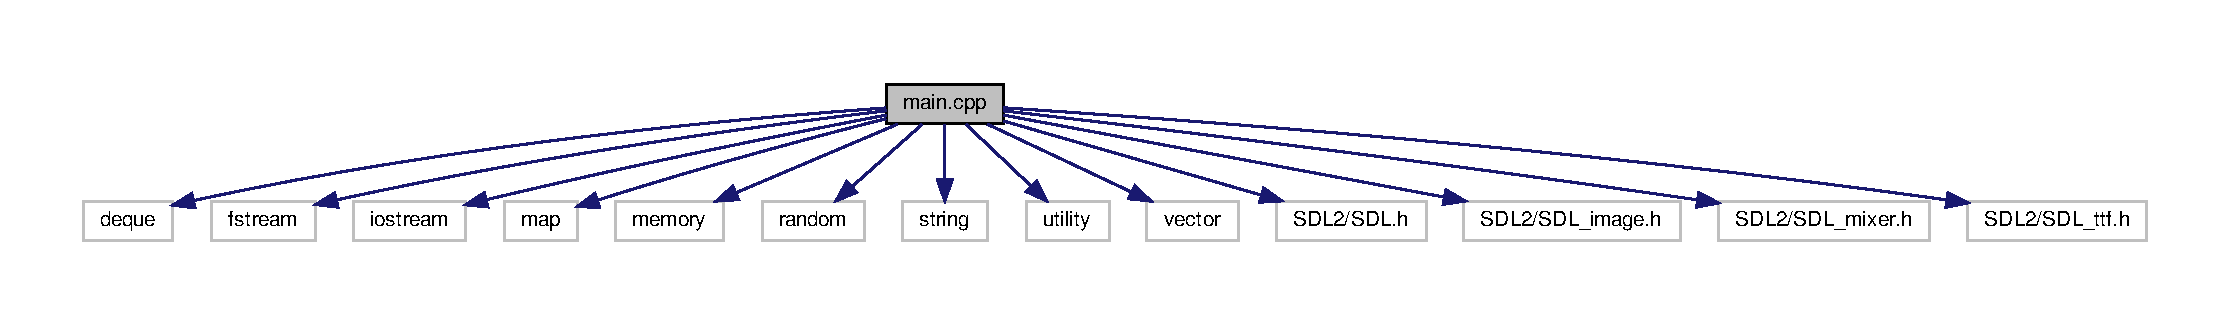
\includegraphics[width=350pt]{main_8cpp__incl}
\end{center}
\end{figure}
\subsection*{Membri}
\begin{DoxyCompactItemize}
\item 
struct \hyperlink{structPunct}{Punct}
\item 
class \hyperlink{classStadiulJocului}{Stadiul\+Jocului}
\begin{DoxyCompactList}\small\item\em Contine toata informatia de care avem nevoie in timpul jocului. \end{DoxyCompactList}\item 
class \hyperlink{classScena}{Scena}
\begin{DoxyCompactList}\small\item\em Interfata pentru toate scenele. \end{DoxyCompactList}\item 
class \hyperlink{classJoc}{Joc}
\begin{DoxyCompactList}\small\item\em \hyperlink{classScena}{Scena} jocului in sine. \end{DoxyCompactList}\item 
class \hyperlink{classMeniuStart}{Meniu\+Start}
\begin{DoxyCompactList}\small\item\em Defineste meniul afisat la deschiderea jocului. \end{DoxyCompactList}\item 
class \hyperlink{classMeniuFinal}{Meniu\+Final}
\begin{DoxyCompactList}\small\item\em Meniul care va fi afisat dupa terminarea unui joc. \end{DoxyCompactList}\end{DoxyCompactItemize}
\subsection*{Namespace-\/uri}
\begin{DoxyCompactItemize}
\item 
 \hyperlink{namespaceglobal}{global}
\end{DoxyCompactItemize}
\subsection*{Enumerări}
\begin{DoxyCompactItemize}
\item 
\mbox{\Hypertarget{main_8cpp_aea66a0d525bf9bfb9b61e9cc1ba0b752}\label{main_8cpp_aea66a0d525bf9bfb9b61e9cc1ba0b752}} 
enum \hyperlink{main_8cpp_aea66a0d525bf9bfb9b61e9cc1ba0b752}{Tip\+Directie} \{ {\bfseries S\+US} = 0, 
{\bfseries J\+OS} = 1, 
{\bfseries S\+T\+A\+N\+GA} = 2, 
{\bfseries D\+R\+E\+A\+P\+TA} = 3
 \}\begin{DoxyCompactList}\small\item\em Unde se poate deplasa omida. \end{DoxyCompactList}
\item 
enum \hyperlink{main_8cpp_a67b02df562611307c1e3adeace56d13e}{Posibilitate\+Teren} \{ {\bfseries G\+OL} = 0, 
{\bfseries O\+M\+I\+DA}, 
{\bfseries F\+R\+U\+N\+ZA}, 
{\bfseries P\+O\+W\+E\+R\+UP}
 \}
\end{DoxyCompactItemize}
\subsection*{Funcţii}
\begin{DoxyCompactItemize}
\item 
\mbox{\Hypertarget{main_8cpp_a9f45632ef14236ddbaf284dc70cd2287}\label{main_8cpp_a9f45632ef14236ddbaf284dc70cd2287}} 
bool \hyperlink{main_8cpp_a9f45632ef14236ddbaf284dc70cd2287}{a\+\_\+apasat} (S\+D\+L\+\_\+\+Scancode tasta)
\begin{DoxyCompactList}\small\item\em Verifica daca jucatorul a apasat tasta data. \end{DoxyCompactList}\item 
void \hyperlink{main_8cpp_af7eff58280fc6fe66098325981310609}{deseneaza\+\_\+cap} (\hyperlink{classStadiulJocului}{Stadiul\+Jocului} \&, int x, int y)
\begin{DoxyCompactList}\small\item\em Deseneaza capul omizii la pozitia data. \end{DoxyCompactList}\item 
\mbox{\Hypertarget{main_8cpp_a45c775a13d22397f62c6a3b31133e01d}\label{main_8cpp_a45c775a13d22397f62c6a3b31133e01d}} 
void \hyperlink{main_8cpp_a45c775a13d22397f62c6a3b31133e01d}{deseneaza\+\_\+corp} (\hyperlink{classStadiulJocului}{Stadiul\+Jocului} \&, int, int)
\begin{DoxyCompactList}\small\item\em Deseneaza un corpul la pozitia data. \end{DoxyCompactList}\item 
\mbox{\Hypertarget{main_8cpp_a413026ec29c72f01082ed5c2235ac9cd}\label{main_8cpp_a413026ec29c72f01082ed5c2235ac9cd}} 
void \hyperlink{main_8cpp_a413026ec29c72f01082ed5c2235ac9cd}{deseneaza\+\_\+frunza} (\hyperlink{classStadiulJocului}{Stadiul\+Jocului} \&)
\begin{DoxyCompactList}\small\item\em Deseneaza frunza. \end{DoxyCompactList}\item 
void \hyperlink{main_8cpp_aa57c630272aa6ab8ab15552adf8c165e}{deseneaza\+\_\+omida} (\hyperlink{classStadiulJocului}{Stadiul\+Jocului} \&)
\begin{DoxyCompactList}\small\item\em Deseneaza intreaga omida. \end{DoxyCompactList}\item 
\mbox{\Hypertarget{main_8cpp_aee9c78f8a1bd879050f1bafc2bb907ce}\label{main_8cpp_aee9c78f8a1bd879050f1bafc2bb907ce}} 
void \hyperlink{main_8cpp_aee9c78f8a1bd879050f1bafc2bb907ce}{deseneaza\+\_\+powerup} (\hyperlink{classStadiulJocului}{Stadiul\+Jocului} \&)
\begin{DoxyCompactList}\small\item\em Deseneaza powerup-\/ul(un mar) pe ecran. \end{DoxyCompactList}\item 
\mbox{\Hypertarget{main_8cpp_ab93314a433d2cc641ea873947bc59df3}\label{main_8cpp_ab93314a433d2cc641ea873947bc59df3}} 
void \hyperlink{main_8cpp_ab93314a433d2cc641ea873947bc59df3}{deseneaza\+\_\+textura} (S\+D\+L\+\_\+\+Texture $\ast$textura, int, int)
\begin{DoxyCompactList}\small\item\em Pune textura data la pozitia data. \end{DoxyCompactList}\item 
\hyperlink{structPunct}{Punct} \hyperlink{main_8cpp_a5f6f5f86af147286478cc7aadd76b0a2}{genereaza\+\_\+pozitie\+\_\+noua} (\hyperlink{classStadiulJocului}{Stadiul\+Jocului} \&stadiu)
\item 
void \hyperlink{main_8cpp_a81cdc1223b468897943076b72f048133}{initializeaza} ()
\item 
void \hyperlink{main_8cpp_a525009107790f4daffd5481e33cb039f}{marcheaza\+\_\+frunza} (\hyperlink{classStadiulJocului}{Stadiul\+Jocului} \&)
\item 
\mbox{\Hypertarget{main_8cpp_ad85beba6ce14e67569c227c8af4d5186}\label{main_8cpp_ad85beba6ce14e67569c227c8af4d5186}} 
void \hyperlink{main_8cpp_ad85beba6ce14e67569c227c8af4d5186}{verifica\+\_\+evenimente} ()
\begin{DoxyCompactList}\small\item\em Vede ce taste a apasat jucatorul si orice alte evenimente. \end{DoxyCompactList}\item 
int \hyperlink{main_8cpp_ae66f6b31b5ad750f1fe042a706a4e3d4}{main} ()
\item 
\mbox{\Hypertarget{main_8cpp_a2f4fa91987e3731c64b385dc822f4425}\label{main_8cpp_a2f4fa91987e3731c64b385dc822f4425}} 
bool {\bfseries e\+\_\+litera} (S\+D\+L\+\_\+\+Scancode t\+\_\+tasta)
\item 
\mbox{\Hypertarget{main_8cpp_a409b453676d92d35f214bc5bacab83d4}\label{main_8cpp_a409b453676d92d35f214bc5bacab83d4}} 
bool {\bfseries e\+\_\+numar} (S\+D\+L\+\_\+\+Scancode t\+\_\+tasta)
\end{DoxyCompactItemize}
\subsection*{Variabile}
\begin{DoxyCompactItemize}
\item 
\hyperlink{structPunct}{Punct} \hyperlink{main_8cpp_a68e903f0d20f0a68b3c01b73eb34e9ed}{directie} \mbox{[}$\,$\mbox{]}
\item 
\mbox{\Hypertarget{namespaceglobal_a07963dc89966c80411e6a3c896c07c10}\label{namespaceglobal_a07963dc89966c80411e6a3c896c07c10}} 
S\+D\+L\+\_\+\+Window $\ast$ \hyperlink{namespaceglobal_a07963dc89966c80411e6a3c896c07c10}{global\+::fereastra} \{ nullptr \}
\begin{DoxyCompactList}\small\item\em Fereastra in care vom desena tot. \end{DoxyCompactList}\item 
S\+D\+L\+\_\+\+Renderer $\ast$ \hyperlink{namespaceglobal_ae80ab1c7d78e562614d35c3b78e44ea3}{global\+::desenator} \{ nullptr \}
\item 
bool \hyperlink{namespaceglobal_a930b1255fa49cd41dc635136822d56ee}{global\+::fereastra\+\_\+inchisa} = false
\item 
\mbox{\Hypertarget{namespaceglobal_a5ad71f80dc82eb6fd1036c8055a5dfbc}\label{namespaceglobal_a5ad71f80dc82eb6fd1036c8055a5dfbc}} 
constexpr int \hyperlink{namespaceglobal_a5ad71f80dc82eb6fd1036c8055a5dfbc}{global\+::lungime} = 600
\begin{DoxyCompactList}\small\item\em Lungimea ferestrei. \end{DoxyCompactList}\item 
\mbox{\Hypertarget{namespaceglobal_a612e7b296f148c02400618f1770f57f7}\label{namespaceglobal_a612e7b296f148c02400618f1770f57f7}} 
constexpr int \hyperlink{namespaceglobal_a612e7b296f148c02400618f1770f57f7}{global\+::inaltime} = 600
\begin{DoxyCompactList}\small\item\em Inaltimea ferestrei. \end{DoxyCompactList}\item 
std\+::deque$<$ std\+::unique\+\_\+ptr$<$ \hyperlink{classScena}{Scena} $>$ $>$ \hyperlink{namespaceglobal_af4564594d950b73d4bb81b8c0a4fe029}{global\+::scene}
\item 
std\+::map$<$ S\+D\+L\+\_\+\+Scancode, bool $>$ \hyperlink{namespaceglobal_a6da5c1308adb9fdac1c61389b139dc54}{global\+::taste\+\_\+apasate}
\end{DoxyCompactItemize}


\subsection{Documentaţia enumerărilor}
\mbox{\Hypertarget{main_8cpp_a67b02df562611307c1e3adeace56d13e}\label{main_8cpp_a67b02df562611307c1e3adeace56d13e}} 
\index{main.\+cpp@{main.\+cpp}!Posibilitate\+Teren@{Posibilitate\+Teren}}
\index{Posibilitate\+Teren@{Posibilitate\+Teren}!main.\+cpp@{main.\+cpp}}
\subsubsection{\texorpdfstring{Posibilitate\+Teren}{PosibilitateTeren}}
{\footnotesize\ttfamily enum \hyperlink{main_8cpp_a67b02df562611307c1e3adeace56d13e}{Posibilitate\+Teren}}

Terenul este o matrice care contine una din urmatoarele posibilitati de mai jos. 

Definiţia în linia 365 a fişierului main.\+cpp.



\subsection{Documentaţia funcţiilor}
\mbox{\Hypertarget{main_8cpp_af7eff58280fc6fe66098325981310609}\label{main_8cpp_af7eff58280fc6fe66098325981310609}} 
\index{main.\+cpp@{main.\+cpp}!deseneaza\+\_\+cap@{deseneaza\+\_\+cap}}
\index{deseneaza\+\_\+cap@{deseneaza\+\_\+cap}!main.\+cpp@{main.\+cpp}}
\subsubsection{\texorpdfstring{deseneaza\+\_\+cap()}{deseneaza\_cap()}}
{\footnotesize\ttfamily void deseneaza\+\_\+cap (\begin{DoxyParamCaption}\item[{\hyperlink{classStadiulJocului}{Stadiul\+Jocului} \&}]{stadiu,  }\item[{int}]{x,  }\item[{int}]{y }\end{DoxyParamCaption})}



Deseneaza capul omizii la pozitia data. 


\begin{DoxyParams}[1]{Parametri}
\mbox{\tt in}  & {\em x} & Coordonata lungime ca in plan cartezian. \\
\hline
\mbox{\tt in}  & {\em y} & Inaltimea, coordonata (0, 0) este in coltul din stanga sus al ferestrei.\\
\hline
\end{DoxyParams}
\begin{DoxyAttention}{Atenţie}
Pozitia data nu are aceleasi coordonate ca \hyperlink{structPunct}{Punct}. x si y se refera la pozitia in fereastra, nu in matrice. Se aplica si la \hyperlink{main_8cpp_a45c775a13d22397f62c6a3b31133e01d}{deseneaza\+\_\+corp}, \hyperlink{main_8cpp_ab93314a433d2cc641ea873947bc59df3}{deseneaza\+\_\+textura}. 
\end{DoxyAttention}


Definiţia în linia 837 a fişierului main.\+cpp.



Referinţe deseneaza\+\_\+textura().



Semnalat de deseneaza\+\_\+omida().

\mbox{\Hypertarget{main_8cpp_aa57c630272aa6ab8ab15552adf8c165e}\label{main_8cpp_aa57c630272aa6ab8ab15552adf8c165e}} 
\index{main.\+cpp@{main.\+cpp}!deseneaza\+\_\+omida@{deseneaza\+\_\+omida}}
\index{deseneaza\+\_\+omida@{deseneaza\+\_\+omida}!main.\+cpp@{main.\+cpp}}
\subsubsection{\texorpdfstring{deseneaza\+\_\+omida()}{deseneaza\_omida()}}
{\footnotesize\ttfamily void deseneaza\+\_\+omida (\begin{DoxyParamCaption}\item[{\hyperlink{classStadiulJocului}{Stadiul\+Jocului} \&}]{stadiu }\end{DoxyParamCaption})}



Deseneaza intreaga omida. 

Parcurge \hyperlink{classStadiulJocului_a64e0608d9c68b22ea83fd5aba209453f}{Stadiul\+Jocului\+::pozitii\+\_\+omida} si deseneaza fiecare parte a omizii. 

Definiţia în linia 853 a fişierului main.\+cpp.



Referinţe deseneaza\+\_\+cap(), deseneaza\+\_\+corp(), Punct\+::i, Stadiul\+Jocului\+::inaltime\+\_\+textura, Punct\+::j, Stadiul\+Jocului\+::lungime\+\_\+textura şi Stadiul\+Jocului\+::pozitii\+\_\+omida.

\mbox{\Hypertarget{main_8cpp_a5f6f5f86af147286478cc7aadd76b0a2}\label{main_8cpp_a5f6f5f86af147286478cc7aadd76b0a2}} 
\index{main.\+cpp@{main.\+cpp}!genereaza\+\_\+pozitie\+\_\+noua@{genereaza\+\_\+pozitie\+\_\+noua}}
\index{genereaza\+\_\+pozitie\+\_\+noua@{genereaza\+\_\+pozitie\+\_\+noua}!main.\+cpp@{main.\+cpp}}
\subsubsection{\texorpdfstring{genereaza\+\_\+pozitie\+\_\+noua()}{genereaza\_pozitie\_noua()}}
{\footnotesize\ttfamily \hyperlink{structPunct}{Punct} genereaza\+\_\+pozitie\+\_\+noua (\begin{DoxyParamCaption}\item[{\hyperlink{classStadiulJocului}{Stadiul\+Jocului} \&}]{stadiu }\end{DoxyParamCaption})}

Returneaza un punct la nimereala cu conditia ca in acea pozitie in matricesa nu fie nimic. 

Definiţia în linia 892 a fişierului main.\+cpp.



Referinţe Punct\+::i, Stadiul\+Jocului\+::inaltime\+\_\+teren, Punct\+::j, Stadiul\+Jocului\+::lungime\+\_\+teren şi Stadiul\+Jocului\+::teren.



Semnalat de Joc\+::itereaza().

\mbox{\Hypertarget{main_8cpp_a81cdc1223b468897943076b72f048133}\label{main_8cpp_a81cdc1223b468897943076b72f048133}} 
\index{main.\+cpp@{main.\+cpp}!initializeaza@{initializeaza}}
\index{initializeaza@{initializeaza}!main.\+cpp@{main.\+cpp}}
\subsubsection{\texorpdfstring{initializeaza()}{initializeaza()}}
{\footnotesize\ttfamily void initializeaza (\begin{DoxyParamCaption}{ }\end{DoxyParamCaption})}

Creeaza fereastra si desenatorul. 

Definiţia în linia 912 a fişierului main.\+cpp.



Referinţe global\+::desenator, global\+::fereastra, global\+::inaltime şi global\+::lungime.



Semnalat de main().

\mbox{\Hypertarget{main_8cpp_ae66f6b31b5ad750f1fe042a706a4e3d4}\label{main_8cpp_ae66f6b31b5ad750f1fe042a706a4e3d4}} 
\index{main.\+cpp@{main.\+cpp}!main@{main}}
\index{main@{main}!main.\+cpp@{main.\+cpp}}
\subsubsection{\texorpdfstring{main()}{main()}}
{\footnotesize\ttfamily int main (\begin{DoxyParamCaption}{ }\end{DoxyParamCaption})}

Toata magia se intampla aici. 

Definiţia în linia 768 a fişierului main.\+cpp.



Referinţe global\+::desenator, global\+::fereastra\+\_\+inchisa, initializeaza(), global\+::scene, global\+::taste\+\_\+apasate, Stadiul\+Jocului\+::timp\+\_\+trecut şi verifica\+\_\+evenimente().

\mbox{\Hypertarget{main_8cpp_a525009107790f4daffd5481e33cb039f}\label{main_8cpp_a525009107790f4daffd5481e33cb039f}} 
\index{main.\+cpp@{main.\+cpp}!marcheaza\+\_\+frunza@{marcheaza\+\_\+frunza}}
\index{marcheaza\+\_\+frunza@{marcheaza\+\_\+frunza}!main.\+cpp@{main.\+cpp}}
\subsubsection{\texorpdfstring{marcheaza\+\_\+frunza()}{marcheaza\_frunza()}}
{\footnotesize\ttfamily void marcheaza\+\_\+frunza (\begin{DoxyParamCaption}\item[{\hyperlink{classStadiulJocului}{Stadiul\+Jocului} \&}]{stadiu }\end{DoxyParamCaption})}

Pune in matricea jocului pe pozitia \hyperlink{classStadiulJocului_a141067404f3678036ee7a91a02532a30}{Stadiul\+Jocului\+::pozitie\+\_\+frunza} Posibilitate\+Teren\+::\+F\+R\+U\+N\+ZA. 

Definiţia în linia 942 a fişierului main.\+cpp.



Referinţe Punct\+::i, Punct\+::j, Stadiul\+Jocului\+::pozitie\+\_\+frunza şi Stadiul\+Jocului\+::teren.



\subsection{Documentaţia variabilelor}
\mbox{\Hypertarget{main_8cpp_a68e903f0d20f0a68b3c01b73eb34e9ed}\label{main_8cpp_a68e903f0d20f0a68b3c01b73eb34e9ed}} 
\index{main.\+cpp@{main.\+cpp}!directie@{directie}}
\index{directie@{directie}!main.\+cpp@{main.\+cpp}}
\subsubsection{\texorpdfstring{directie}{directie}}
{\footnotesize\ttfamily \hyperlink{structPunct}{Punct} directie\mbox{[}$\,$\mbox{]}}

{\bfseries Valoarea iniţială\+:}
\begin{DoxyCode}
= \{
    \{ -1,  0 \}, 
    \{  1,  0 \}, 
    \{  0, -1 \}, 
    \{  0,  1 \}  
\}
\end{DoxyCode}
Pentru a face mutarea omizii mai usoara pozitiile capului si cozii vor fi actualizate cu pozitiile lor curente + directie\mbox{[}S\+T\+A\+N\+GA\mbox{]} sau D\+R\+E\+A\+P\+TA etc. 
\begin{DoxyCode}
\hyperlink{structPunct}{Punct} cap\{ 2, 3 \};
\textcolor{comment}{// Pentru a muta la stanga:}
cap.\hyperlink{structPunct_a28bb6f2facdfadbf7e19d651c526a646}{i} += \hyperlink{main_8cpp_a68e903f0d20f0a68b3c01b73eb34e9ed}{directie}[STANGA].\hyperlink{structPunct_a28bb6f2facdfadbf7e19d651c526a646}{i};
cap.j += \hyperlink{main_8cpp_a68e903f0d20f0a68b3c01b73eb34e9ed}{directie}[STANGA].\hyperlink{structPunct_a065a30931a1d15d6f6c638c4888d254e}{j};
\end{DoxyCode}
 

Definiţia în linia 355 a fişierului main.\+cpp.


%--- End generated contents ---

% Index
\backmatter
\newpage
\phantomsection
\clearemptydoublepage
\addcontentsline{toc}{chapter}{Index}
\printindex

\end{document}
